\setcounter{secnumdepth}{3}
\section{Panoramica}
GameUp è un software dedicato a due tipi di utenti finali: videogiocatori e sviluppatori di videogiochi. Il sistema deve offrire un insieme di funzionalità base per tutti gli utenti, oltre che a funzionalità specifiche per le singole specializzazioni.
In particolare, le funzionalità base da offrire sono:
\begin{itemize}
\item Mostrare un catalogo di videogiochi attualmente attivi nella piattaforma, mostrando delle informazioni di base ed offrendo dettagli aggiuntivi come descrizione, immagini di esempio e recensioni al click dell’utente;
\item Permettere l’acquisto di un videogioco dalla pagina del dettaglio di esso;
\item Permettere funzionalità di autenticazione (registrazione e log-in) per rendere più semplice l’interazione con la piattaforma, salvando il metodo di pagamento o permettendo la stesura di una recensione, o di avere accesso a funzionalità dedicate agli sviluppatori o agli amministratori;
\item Filtrare il catalogo per trovare giochi inerenti ai gusti dell’utente, o per rimuovere giochi indesiderati;
\end{itemize}
Mentre le funzionalità aggiuntive dedicate agli sviluppatori sono:
\begin{itemize}
\item Richiedere l’aggiunta del proprio videogioco all’interno della piattaforma compilando un modulo contenente le informazioni necessarie;
\item Gestire i propri videogiochi pubblicati, modificandone le informazioni;
\item Gestire il forum dedicato al proprio videogioco, dando la possibilità di creare una comunità affiatata e di rispondere ad eventuali domande poste dagli utenti;
\end{itemize}
Infine, le funzionalità aggiuntive degli amministratori della piattaforma sono:
\begin{itemize}
\item Avere il controllo totale della piattaforma, potendo quindi modificare le informazioni di qualsiasi videogioco, per poter moderare le informazioni dove necessario;
\item Approvare o negare le richieste di inserimento di videogiochi da parte degli sviluppatori;
\item Gestire eventuali problemi sotto forma di ticket da parte degli utenti;
\item Poter moderare le comunità dei vari videogiochi, in particolare potendo cancellare eventuali messaggi o recensioni con contenuti dannosi, come ad esempio lo spam;
\end{itemize}

\section{Identificazione degli attori}
\begin{center}
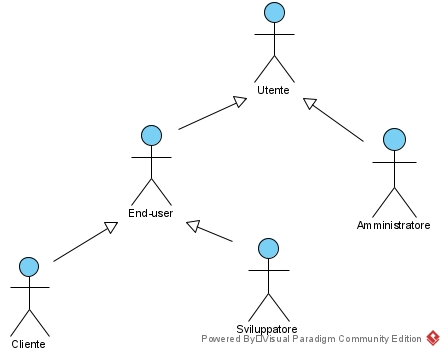
\includegraphics{Figure/actorsDiagram.jpg}
\end{center}

\section{Requisiti funzionali}
La priorità di ogni requisito è indicata prima dell'identificativo, tra parentesi.
\subsection{RF Gestione Account (Utenti)}
\begin{enumerate}
	\item \textbf{(Alta) Registrazione}: Un utente non registrato deve poter registrarsi alla piattaforma;
	\item \textbf{(Alta) Log-in}: L’utente registrato deve poter immettere le sue credenziali per potersi autenticare;
	\item \textbf{(Alta) Logout}: L’utente autenticato deve poter uscire dalla piattaforma;
	\item \textbf{(Alta) Visualizza profilo}: L’utente autenticato deve poter visualizzare le informazioni collegate al suo account;
	\item \textbf{(Alta) Modifica Profilo}: L’utente autenticato deve poter modificare le informazioni relative al suo account. In particolare, deve poter segnare l’opzione Sviluppatore per diventare uno Sviluppatore;
	\item \textbf{(Bassa) Recupera Password}: L’utente registrato deve poter richiedere il reset della password nel caso se ne sia dimenticato;
	\item \textbf{(Media) Chiusura Discussione}: Un utente deve poter essere in grado di chiudere una discussione, la propria se è un cliente, una relativa al proprio videogioco se è uno sviluppatore oppure tutte nel caso di un amministratore.
\end{enumerate}

\subsection{RF End-user}
\begin{enumerate}
	\item \textbf{(Media) Creazione Discussione}: Un end-user deve poter creare una discussione all’interno del forum dedicato ad un particolare videogioco.
	\item \textbf{(Media) Commento Discussione}: Un end-user deve poter commentare in una discussione esistente, nel caso non sia chiusa.
	\item \textbf{(Media) Visualizzazione Comunità Videogioco}: Il visitatore deve poter visualizzare il forum dedicato ad un determinato videogioco, formato da discussioni contenenti messaggi scritti da utenti autenticati, in particolare dagli autori del videogioco;
	\item \textbf{(Bassa) Report Contenuto}: Un end-user deve poter segnalare un particolare contenuto (un videogioco o un commento) come offensivo, per richiedere agli amministratori del sistema la sua rimozione;
\end{enumerate}

\subsection{RF Clienti}
\begin{enumerate}
	\item \textbf{(Alta) Visualizzazione Pagina Iniziale}: Il cliente deve poter visualizzare una vetrina di videogiochi selezionati secondo vari criteri dal sistema;
	\item \textbf{(Alta) Visualizzazione Catalogo}: Il cliente deve poter visualizzare il catalogo di tutti i videogiochi attivi della piattaforma, ovvero i dettagli sostanziali che lo descrivono come nome, prezzo, autore e logo, avendo la possibilità di filtrarli secondo determinati criteri;
	\item \textbf{(Alta) Visualizzazione Dettagli Videogioco}: Il cliente deve poter visualizzare i dettagli relativi ad un particolare videogioco, come ad esempio la descrizione per esteso, la versione, immagini di anteprima e le recensioni;
	\item \textbf{(Alta) Acquisto Videogioco}: Il cliente autenticato deve poter effettuare il download del gioco scelto dalla sua schermata dei dettagli, nel caso sia gratis, oppure previo pagamento. In particolare, deve poter avere la possibilità di scegliere la versione da scaricare;
	\item \textbf{(Media) Recensione Videogioco}: se lo consiglierebbe ad un amico ed eventuali note aggiuntive lasciate come testo;
	\item \textbf{(Media) Valutazione Recensione}: Il cliente autenticato deve poter valutare una singola recensione in maniera positiva o negativa.
	\item \textbf{(Media) Suggerimento Tags}: Il cliente autenticato deve poter suggerire ulteriori tag per un videogioco acquistato, scegliendone una tra le più popolari del momento oppure fornendo una propria tag come suggerimento.	
\end{enumerate}

\subsection{RF Sviluppatori}
\begin{enumerate}
	\item \textbf{(Alta) Richiesta Inserimento Videogioco}: Lo sviluppatore deve poter accedere ad un modulo compilabile, tramite il quale può richiedere agli amministratori della piattaforma la pubblicazione del proprio videogioco;
	\item \textbf{(Media) Messa in Rilievo di una Discussione}: Lo sviluppatore deve poter fissare come discussione importante una o più discussioni contenute all’interno del forum dedicato ad un videogioco pubblicato da lui.
	\item \textbf{(Media) Richiesta di Modifica Dati Videogioco}: Lo sviluppatore deve poter modificare le informazioni relative ad un gioco da lui pubblicato. In particolare, deve poter caricare una nuova versione del suo videogioco (un aggiornamento), senza però sovrascrivere le versioni esistenti, le quali rimangono pubbliche e scaricabili.
	\item \textbf{(Media) Sponsorizzazione Videogioco}: Lo sviluppatore deve poter sponsorizzare un proprio videogioco, specificando le settimane durante le quali applicare i privilegi della sponsorizzazione, tra quelle mostrate come disponibili dal sistema previo pagamento.	
\end{enumerate}

\subsection{RF Amministratori}
\begin{enumerate}
	\item \textbf{(Media) Risoluzione richieste pubblicazione/modifica videogiochi}: L’amministratore deve poter accettare o rifiutare una richiesta di pubblicazione o di modifica di un videogioco.
	\\Nel caso di una approvazione, il sistema provvede a creare e rendere pubblica la schermata di dettaglio del videogioco basandosi sui dati forniti dallo sviluppatore nel modulo da lui pubblicato.
	\item \textbf{(Media) Modifica dati videogioco}: L’amministratore deve poter modificare immediatamente i dati relativi ad un videogioco, direttamente dalla pagina dei dettagli di tale, senza dover richiedere l’approvazione di un altro amministratore.
	\item \textbf{(Bassa) Rimozione contenuto offensivo}: L’amministratore deve poter nascondere contenuti pubblici di qualsiasi tipo, come ad esempio videogiochi, commenti o discussioni nocive e recensioni per il bene della piattaforma;
	\item \textbf{(Bassa) Risoluzione report}: L’amministratore deve poter marcare un report come risolto, sia in maniera positiva oppure negativa, così che il sistema possa avvisare automaticamente gli utenti relativi ad un determinato report delle azioni eseguite dall’amministratore per la risoluzione.	
\end{enumerate}

\section{Requisiti non funzionali}
\subsection{(Alta) Usabilità}
Il sistema deve essere accessibile da qualsiasi piattaforma, in particolare per i dispositivi mobile, ovvero i target principali del sistema. Opzionalmente, deve essere accessibile anche da dispositivi non mobile, come ad esempio un desktop, principalmente per rendere più semplice l’uso per gli sviluppatori e gli amministratori. I contenuti caricati dagli sviluppatori devono seguire un format standard, così da non confondere gli utenti durante la navigazione del catalogo.

\subsection{(Alta) Affidabilità}
Il sottosistema di autenticazione degli utenti registrati deve essere robusto, basandosi su un algoritmo di sicurezza valido e gli utenti devono avere accesso solo specificatamente alle risorse necessarie, nella modalità necessaria (solo lettura o lettura e scrittura). Gli sviluppatori devono avere più permessi di un normale utente registrato, ma solo per le pagine relative ai loro videogiochi, senza poter impersonare o abusare, però, altri utenti o altri videogiochi, ad esempio nel forum non devono poter cancellare i contenuti altrui, per evitare la cancellazione di feedback negativi validi, mentre le richieste di aggiunta o modifica del proprio videogioco devono necessariamente passare per un controllo di validazione da parte degli amministratori, per evitare contenuti atti a danneggiare la piattaforma.

\subsection{(Media) Performance}
Il sistema deve poter soddisfare le richieste di svariati utenti, utilizzando servizi moderni per la distribuzione di contenuti. In particolare, il download e l’upload dei videogiochi non devono impattare la visualizzazione del sito, essendo l’operazione più onerosa del sistema.

\subsection{(Media) Manutenibilità}
Il sistema deve essere dotato dei test necessari per garantire, in primis, che la parte dedicata agli utenti finali non subisca danni durante gli aggiornamenti del sistema, per evitare aggiornamenti dannosi.

\subsection{(Media) Legali}
I dati personali degli utenti registrati devono essere trattati secondo le regole definite dal Regolamento Ue 2016/679, noto come GDPR. La cancellazione di un videogioco dal sistema da parte degli amministratori deve essere possibile nel caso di problemi legali derivanti da quel videogioco, ad esempio se uno sviluppatore pubblica un videogioco non realizzato da lui. Inoltre, i pagamenti all’interno della piattaforma vengono processati con un servizio esterno, per garantire la sicurezza dei dati, per poi essere divisi con i singoli sviluppatori mantenendo una determinata percentuale pattuita dal contratto firmato dalla società del sistema GameUp e lo sviluppatore di un videogioco inserito. 

\section{Modello del sistema}
\subsection{Scenari}
	\small\begin{tabular}{|| l | p{30em} ||} 
	\hline
	Nome Scenario & Registrazione di un cliente\\
	\hline
	Partecipanti & Bob: utente non registrato con dispositivo Android\\
	\hline
	Descrizione & Lo scenario descrive la scoperta, da parte di Bob, della piattaforma GameUp. Bob decide di registrarsi per avere accesso ad ulteriori funzionalità, così da poter trovare il gioco perfetto per il suo smartphone.\\
	\hline
	Vantaggi & Il cliente non registrato Bob diventa un cliente registrato, così da poter effettivamente effettuare l’acquisto di un videogioco.\\
	\hline
	Flusso degli eventi &
	\begin{enumerate}
		\item Bob, tramite il suo smartphone Android, decide di cercare un nuovo videogioco per occupare il suo tempo libero. Non riesce a trovare un videogioco soddisfacente sullo store ufficiale, pieno di applicazioni di bassa qualità, quindi decide di provare GameUp.
		\item Bob accede alla piattaforma GameUp ed inizia a controllare la vetrina principale con i videogiochi in evidenza. Trova un gioco che gli interessa dopo aver visualizzato i dettagli, ma nota che deve registrarsi per effettuare il download.
		\item Bob va sulla schermata di log-in, scegliendo come opzione “Registrati”, e compila username, e-mail e password e conferma password, per poi procedere.
		\item Il sistema acquisisce i dati di Bob, controllando che non ci siano collisioni con username o e-mail. In caso di successo, Bob viene inserito all’interno del sistema, altrimenti viene avvisato del conflitto, attendendo ulteriori dati da Bob.
		\item Bob riesce a registrarsi e viene automaticamente autorizzato dal sistema, così da poter effettuare il download del videogioco scelto.
	\end{enumerate} \\
	\hline
	\end{tabular}

	\small\begin{tabular}{|| l | p{30em} ||} 
	\hline
	Nome Scenario & Log-in e log-out\\
	\hline
	Partecipanti & Bob: cliente registrato con dispositivo Android\\
	\hline
	Descrizione & Lo scenario descrive il ritorno di Bob sulla piattaforma GameUp, dopo essersi divertito con il videogioco precedentemente installato.\\
	\hline
	Vantaggi & Il cliente Bob viene autorizzato dal sistema, così da poter avere più funzionalità a sua disposizione, per poi effettuare il log-out per evitare che suo figlio esegua erroneamente il pagamento per qualche videogioco.\\
	\hline
	Flusso degli eventi &
	\begin{enumerate}
		\item Bob torna sulla piattaforma GameUp, selezionando la schermata di log-in.
		\item Bob inserisce il suo username e la sua password, mandandole al sistema.
		\item Il sistema autentica Bob.
		\item Bob controlla il catalogo per vedere se riesce a trovare qualche videogioco interessante.
		\item Bob decide di non scaricare nulla, quindi nella stessa posizione del pulsante che permette il log-in, trova il pulsante log-out, lo clicca ed effettua il log-out.
		\item La sessione viene invalidata dal sistema e il log-out di Bob viene eseguito.
		\item Bob dà il suo smartphone a Bob Jr., il quale prontamente prova a comprare un gioco da 60€ accidentalmente, fallendo poiché non è attualmente un utente autenticato.
	\end{enumerate} \\
	\hline
	\end{tabular}

	\small\begin{tabular}{|| l | p{30em} ||} 
	\hline
	Nome Scenario & Attacco hacker ai dati di un visitatore\\
	\hline
	Partecipanti & Bob: cliente registrato con dispositivo Android\\
	\hline
	Descrizione & Lo scenario descrive la scoperta, da parte di Bob, dell’esposizione del suo username e della sua password che usa per tutti i servizi online, GameUp incluso, mostrando gli scenari di recupero password, visualizzazione e modifica del profilo.\\
	\hline
	Vantaggi & L’utente registrato Bob è in grado di entrare nuovamente in possesso del suo profilo, cambiando i dati personali salvati.\\
	\hline
	Flusso degli eventi &
	\begin{enumerate}
		\item Bob, tramite il suo smartphone Android, scopre di essere stato vittima di un attacco hacker. Dopo aver resettato i suoi dati sui vari servizi in uso, decide di provare ad entrare nella piattaforma GameUp, fallendo.
		\item Il sistema continua a dare un errore di password errata, così Bob decide di richiedere il reset della password tramite l’apposito link sotto il modulo per il log-in.
		\item Il sistema visualizza una pagina con un semplice modulo il quale richiede l’inserimento della e-mail.
		\item Bob inserisce l’e-mail collegata al suo account.
		\item Il sistema processa la richiesta, inviando una e-mail all’indirizzo fornito (nel caso sia un indirizzo effettivamente valido ed associato ad un profilo) contenente un link temporaneo per il reset della password.
		\item Bob naviga su questo link temporaneo, dove gli viene mostrato un modulo per il cambio della password.
		\item Bob cambia la sua password con successo, decidendo di visualizzare il suo profilo per vedere se i suoi dati sono stati cambiati dall’attaccante hacker.
		\item Il sistema fornisce una semplice vista dei dati di Bob, ovvero username, e-mail, password e se il suo account è un account sviluppatore, e Bob nota che il suo username è stato cambiato.
		\item Bob clicca su un pulsante che abilita la modifica dei dati visualizzati e decide di ripristinare l’username.
		\item Il sistema accoglie la richiesta di Bob, aggiornando i suoi dati.
	\end{enumerate} \\
	\hline
	\end{tabular}

	\small\begin{tabular}{|| l | p{30em} ||} 
	\hline
	Nome Scenario & Scoperta di un videogioco interessante\\
	\hline
	Partecipanti & Tim: cliente registrato con dispositivo Android\\
	\hline
	Descrizione & Lo scenario descrive la scoperta, da parte di Tim, di un videogioco che corrisponde perfettamente ai suoi criteri, grazie alle funzionalità offerte dalla piattaforma. Tim è un perfezionista e decide di controllare accuratamente i dettagli del videogioco prima di effettuarne il download.\\
	\hline
	Vantaggi & Questo scenario mostra il classico uso di un videogiocatore della piattaforma GameUp.\\
	\hline
	Flusso degli eventi &
	\begin{enumerate}
		\item Il giovane Tim ha bisogno di un videogioco che lo soddisfi e che gli permetta di spendere svariate ore su di esso.
		\item Tim controlla le categorie visualizzabili dalla vetrina ma non nota nulla che lo interessi.
		\item Tim decide, quindi, di andare direttamente sul catalogo, dove gli vengono offerti vari filtri di ricerca per trovare il videogioco perfetto per lui.
		\item Egli sceglie come filtri un videogioco di tipo gestionale, ma che sia solo multiplayer e a tema steampunk oppure sci-fi. Inoltre, vuole che il videogioco sia in beta, così da poter diventare uno dei giocatori migliori e avere un vantaggio sui giocatori futuri.
		\item Il sistema esegue una ricerca all’interno del database, ritornando tutti i giochi che rispettano le caratteristiche fornite da Tim, in modo sia esclusivo (il gioco deve essere sia multiplayer, sia in beta) che opzionale (il gioco deve essere di genere steampunk oppure sci-fi)
		\item Tim inizia a controllare i vari risultati, andando nelle pagine dei dettagli di ogni videogioco. In particolare, controlla le recensioni degli altri utenti, controllando il punteggio medio e le note delle recensioni più votate.
		\item Tim trova un videogioco molto amato dai suoi videogiocatori e decide di scaricare l’ultima versione, procedendo prima ad effettuare il log-in, selezionandola dopo aver premuto il pulsante di download. Tim scopre che il videogioco è di suo gradimento e decide di lasciare una semplice recensione positiva, valutando positivamente anche le recensioni che lo hanno aiutato a scegliere il videogioco.			
	\end{enumerate} \\
	\hline
	\end{tabular}

	\small\begin{tabular}{|| l | p{30em} ||} 
	\hline
	Nome Scenario & Scoperta di un videogioco interessante\\
	\hline
	Partecipanti & Tim: cliente registrato con dispositivo Android\\
	\hline
	Descrizione & Lo scenario descrive la scoperta, da parte di Tim, di un videogioco che corrisponde perfettamente ai suoi criteri, grazie alle funzionalità offerte dalla piattaforma. Tim è un perfezionista e decide di controllare accuratamente i dettagli del videogioco prima di effettuarne il download.\\
	\hline
	Vantaggi & Questo scenario mostra il classico uso di un videogiocatore della piattaforma GameUp.\\
	\hline
	Flusso degli eventi &
	\begin{enumerate}
		\item Il giovane Tim ha bisogno di un videogioco che lo soddisfi e che gli permetta di spendere svariate ore su di esso.
		\item Tim controlla le categorie visualizzabili dalla vetrina ma non nota nulla che lo interessi.
		\item Tim decide, quindi, di andare direttamente sul catalogo, dove gli vengono offerti vari filtri di ricerca per trovare il videogioco perfetto per lui.
		\item Egli sceglie come filtri un videogioco di tipo gestionale, ma che sia solo multiplayer e a tema steampunk oppure sci-fi. Inoltre, vuole che il videogioco sia in beta, così da poter diventare uno dei giocatori migliori e avere un vantaggio sui giocatori futuri.
		\item Il sistema esegue una ricerca all’interno del database, ritornando tutti i giochi che rispettano le caratteristiche fornite da Tim, in modo sia esclusivo (il gioco deve essere sia multiplayer, sia in beta) che opzionale (il gioco deve essere di genere steampunk oppure sci-fi)
		\item Tim inizia a controllare i vari risultati, andando nelle pagine dei dettagli di ogni videogioco. In particolare, controlla le recensioni degli altri utenti, controllando il punteggio medio e le note delle recensioni più votate.
		\item Tim trova un videogioco molto amato dai suoi videogiocatori e decide di scaricare l’ultima versione, procedendo prima ad effettuare il log-in, selezionandola dopo aver premuto il pulsante di download. Tim scopre che il videogioco è di suo gradimento e decide di lasciare una semplice recensione positiva, valutando positivamente anche le recensioni che lo hanno aiutato a scegliere il videogioco.			
	\end{enumerate} \\
	\hline
	\end{tabular}

	\small\begin{tabular}{|| l | p{30em} ||} 
	\hline
	Nome Scenario & Scoperta di un videogioco interessante\\
	\hline
	Partecipanti & Tim: cliente registrato con dispositivo Android\\
	\hline
	Descrizione & Lo scenario descrive la scoperta, da parte di Tim, di un videogioco che corrisponde perfettamente ai suoi criteri, grazie alle funzionalità offerte dalla piattaforma. Tim è un perfezionista e decide di controllare accuratamente i dettagli del videogioco prima di effettuarne il download.\\
	\hline
	Vantaggi & Questo scenario mostra il classico uso di un videogiocatore della piattaforma GameUp.\\
	\hline
	Flusso degli eventi &
	\begin{enumerate}
		\item Il giovane Tim ha bisogno di un videogioco che lo soddisfi e che gli permetta di spendere svariate ore su di esso.
		\item Tim controlla le categorie visualizzabili dalla vetrina ma non nota nulla che lo interessi.
		\item Tim decide, quindi, di andare direttamente sul catalogo, dove gli vengono offerti vari filtri di ricerca per trovare il videogioco perfetto per lui.
		\item Egli sceglie come filtri un videogioco di tipo gestionale, ma che sia solo multiplayer e a tema steampunk oppure sci-fi. Inoltre, vuole che il videogioco sia in beta, così da poter diventare uno dei giocatori migliori e avere un vantaggio sui giocatori futuri.
		\item Il sistema esegue una ricerca all’interno del database, ritornando tutti i giochi che rispettano le caratteristiche fornite da Tim, in modo sia esclusivo (il gioco deve essere sia multiplayer, sia in beta) che opzionale (il gioco deve essere di genere steampunk oppure sci-fi)
		\item Tim inizia a controllare i vari risultati, andando nelle pagine dei dettagli di ogni videogioco. In particolare, controlla le recensioni degli altri utenti, controllando il punteggio medio e le note delle recensioni più votate.
		\item Tim trova un videogioco molto amato dai suoi videogiocatori e decide di scaricare l’ultima versione, procedendo prima ad effettuare il log-in, selezionandola dopo aver premuto il pulsante di download. Tim scopre che il videogioco è di suo gradimento e decide di lasciare una semplice recensione positiva, valutando positivamente anche le recensioni che lo hanno aiutato a scegliere il videogioco.			
	\end{enumerate} \\
	\hline
	\end{tabular}

\small\begin{tabular}{|| l | p{30em} ||} 
	\hline
	Nome Scenario & Attacco hacker ai dati di un visitatore\\
	\hline
	Partecipanti & Bob: cliente registrato con dispositivo Android\\
	\hline
	Descrizione & Lo scenario descrive la scoperta, da parte di Bob, dell’esposizione del suo username e della sua password che usa per tutti i servizi online, GameUp incluso, mostrando gli scenari di recupero password, visualizzazione e modifica del profilo.\\
	\hline
	Vantaggi & L’utente registrato Bob è in grado di entrare nuovamente in possesso del suo profilo, cambiando i dati personali salvati.\\
	\hline
	Flusso degli eventi &
	\begin{enumerate}
		\item Bob, tramite il suo smartphone Android, scopre di essere stato vittima di un attacco hacker. Dopo aver resettato i suoi dati sui vari servizi in uso, decide di provare ad entrare nella piattaforma GameUp, fallendo.
		\item Il sistema continua a dare un errore di password errata, così Bob decide di richiedere il reset della password tramite l’apposito link sotto il modulo per il log-in.
		\item Il sistema visualizza una pagina con un semplice modulo il quale richiede l’inserimento della e-mail.
		\item Bob inserisce l’e-mail collegata al suo account.
		\item Il sistema processa la richiesta, inviando una e-mail all’indirizzo fornito (nel caso sia un indirizzo effettivamente valido ed associato ad un profilo) contenente un link temporaneo per il reset della password.
		\item Bob naviga su questo link temporaneo, dove gli viene mostrato un modulo per il cambio della password.
		\item Bob cambia la sua password con successo, decidendo di visualizzare il suo profilo per vedere se i suoi dati sono stati cambiati dall’attaccante hacker.
		\item Il sistema fornisce una semplice vista dei dati di Bob, ovvero username, e-mail, password e se il suo account è un account sviluppatore, e Bob nota che il suo username è stato cambiato.
		\item Bob clicca su un pulsante che abilita la modifica dei dati visualizzati e decide di ripristinare l’username.
		\item Il sistema accoglie la richiesta di Bob, aggiornando i suoi dati.
	\end{enumerate} \\
	\hline
	\end{tabular}

	\small\begin{tabular}{|| l | p{30em} ||} 
	\hline
	Nome Scenario & Suggerimento tag videogioco\\
	\hline
	Partecipanti & Tim: cliente con dispositivo Android\\
	\hline
	Descrizione & Lo scenario descrive il suggerimento di una tag per un videogioco da parte di un cliente che possiede tale videogioco.\\
	\hline
	Vantaggi & Le tag suggerite dagli utenti vengono mostrate nella descrizione del videogioco e possono essere usate come criterio di ricerca di un videogioco.\\
	\hline
	Flusso degli eventi &
	\begin{enumerate}
		\item Tim ha acquistato un videogioco e, dopo aver giocato per un po’ di tempo, nota che sulla pagina dei dettagli del videogioco non è indicata la tag “PvE” come caratteristica del videogioco.
		\item Tim naviga sulla pagina del videogioco, cliccando sulla + vicina alla sezione relativa alle tag.
		\item Il sistema mostra a Tim un elenco delle 20 tag più popolari consigliate dagli utenti, assieme ad un semplice campo testuale per inserire la tag voluta.
		\item Tim nota una tag popolare ma non ancora visibile dalla pagina dei dettagli del videogioco nell’elenco e la clicca.
		\item Il sistema inserisce automaticamente il voto di Tim relativo alla tag popolare scelta.
		\item Tim, inoltre, non nota la tag “PvE” nella lista delle tag popolari, quindi la scrive nel campo testuale, per poi aggiungerla.
		\item Il sistema nota che non esiste una tag di questo tipo, quindi provvede ad aggiungerla segnando Tim come unico voto attualmente esistente.
	\end{enumerate} \\
	\hline
	\end{tabular}

	\small\begin{tabular}{|| l | p{30em} ||} 
	\hline
	Nome Scenario & Conversazione su un forum di un videogioco\\
	\hline
	Partecipanti & Tim: cliente con dispositivo Android\\
	\hline
	Descrizione & Lo scenario descrive l’uso del forum di un videogioco da parte di Tim, il quale ha appena scaricato il videogioco in questione.\\
	\hline
	Vantaggi & Questo scenario dimostra l’utilità del forum per la creazione di una comunità e per dare un luogo di ritrovo per le persone con un interesse in comune, ovvero il videogioco.\\
	\hline
	Flusso degli eventi &
	\begin{enumerate}
		\item Tim, dopo aver scaricato un videogioco gestionale, decide di vedere il forum della comunità di tale videogioco così da trovare possibili alleati e altre persone con cui giocare attraverso una discussione creata da lui.
		\item Tim naviga nella pagina dei dettagli del videogioco scaricato, per poi cliccare il link per andare al forum del videogioco.
		\item Tim decide di iniziare una nuova discussione tramite l’apposito pulsante, specificando il titolo e il messaggio iniziale, per cercare altre persone con cui giocare.
		\item Altre persone iniziano a commentare la discussione di Tim, dando la propria disponibilità per una partita multigiocatore.
		\item Tim risponde tramite l’apposito modulo nella pagina dei dettagli della sua discussione, dichiarando di aver trovato le persone con cui giocare.
		\item Tim decide di chiudere la discussione, avendo raggiunto il suo obiettivo, tramite l’apposito pulsante.
	\end{enumerate} \\
	\hline
	\end{tabular}

	\small\begin{tabular}{|| l | p{30em} ||} 
	\hline
	Nome Scenario & Richiesta di inserimento di un videogioco e modifica\\
	\hline
	Partecipanti & Jim: cliente autenticato, developer di videogiochi indie;
	Bob: cliente autenticato;\\
	\hline
	Descrizione & Lo scenario mostra come un cliente autenticato può diventare sviluppatore e richiedere la pubblicazione del suo videogioco agli amministratori, oltre che a mostrare la modifica dei dettagli di esso e una conversazione tipo tra uno sviluppatore ed un cliente autenticato.\\
	\hline
	Vantaggi & Jim pubblica il suo videogioco sulla piattaforma, arricchendo l’assortimento di videogiochi offerti agli utenti finali.\\
	\hline
	Flusso degli eventi &
	\begin{enumerate}
		\item Jim si accorge che può richiedere, in modo semplice, l’aggiunta del suo videogioco multipiattaforma sviluppato interamente da lui alla piattaforma GameUp, che sta usando da qualche mese.
		\item Jim va nel suo profilo, modificandolo in modo da impostare l’opzione “Sviluppatore” su Si.
		\item Il sistema converte il profilo di Jim in un profilo sviluppatore, dando l’accesso al modulo per la richiesta di pubblicazione di un videogioco.
		\item Jim nota questa nuova opzione, navigandoci, ed inizia a riempire i dati relativi al suo videogioco, fornendo il nome, il logo, alcune immagini di anteprima, una descrizione dettagliata e il videogioco stesso. Inoltre, fornisce un insieme iniziale di caratteristiche che descrivono il suo videogioco: single player, RPG, azione, avventura, open world.
		\item Il sistema inserisce la richiesta in una coda visibile agli amministratori ed eventualmente la richiesta viene approvata.
		\item Il gioco, dopo del tempo, diventa pubblico, ma Jim si accorge di un errore di battitura nella descrizione. Entra nel pannello di modifica, aggiustando l’errore, ed invia una richiesta di aggiornamento.
		\item Un amministratore approva la semplice richiesta di aggiornamento e Jim inizia a vedere le prime recensioni positive.
		\item Bob, uno dei primi giocatori, nota un problema nel videogioco e provvede subito a segnalarlo nella comunità dedicata all’interno della piattaforma.
		\item Jim si accorge della discussione ed assicura Bob che il problema verrà risolto nella prossima versione.
		\item Bob ringrazia e Jim chiude la discussione tramite l’apposito pulsante.
	\end{enumerate} \\
	\hline
	\end{tabular}

	\small\begin{tabular}{|| l | p{30em} ||} 
	\hline
	Nome Scenario & Sponsorizzazione di un videogioco\\
	\hline
	Partecipanti & Jim: sviluppatore di un videogioco attualmente presente nel sistema.\\
	\hline
	Descrizione & Lo scenario descrive il processo per sponsorizzare il proprio videogioco, rendendolo visibile in una categoria apposita nella vetrina della pagina principale del sistema.\\
	\hline
	Vantaggi & Il videogioco risulta immediatamente visibile agli utenti, ad un costo. Il sistema genera una entrata economica di un bene di consumo.\\
	\hline
	Flusso degli eventi &
	\begin{enumerate}
		\item Jim nota che le vendite del suo videogioco sono ancora troppo basse, poiché non ha una comunità stabile appassionata.
		\item Jim naviga nella pagina dei dettagli del suo videogioco, selezionando l’opzione “Sponsorizza”.
		\item Jim indica un insieme di periodi, ovvero settimane, nei quali vuole che il suo gioco venga sponsorizzato. Solo i periodi disponibili vengono visualizzati, ovvero quelli non aventi più di dieci sponsorizzazioni.
		\item Selezionando i periodi, viene indicato il costo della sponsorizzazione.
		\item Jim procede con il pagamento attraverso il servizio esterno.
		\item Una volta che il pagamento è andato a buon fine, la richiesta viene automaticamente approvata.
		\item Durante le settimane indicate, il videogioco di Jim apparirà nella sezione apposita all’interno della pagina principale.		
	\end{enumerate} \\
	\hline
	\end{tabular}

	\small\begin{tabular}{|| l | p{30em} ||} 
	\hline
	Nome Scenario & Risoluzione di una richiesta di pubblicazione o modifica\\
	\hline
	Partecipanti & Frank: amministratore della piattaforma GameUp,
	Jim: sviluppatore\\
	\hline
	Descrizione & Lo scenario descrive l’operazione principale svolta da un amministratore.\\
	\hline
	Vantaggi & L’amministratore ha la possibilità di vedere e accettare o rifiutare le richieste di aggiunta o modifica di videogiochi.\\
	\hline
	Flusso degli eventi &
	\begin{enumerate}
		\item Frank effettua il log-in nella piattaforma GameUp, andando a vedere nell’area riservata agli amministratori le richieste odierne di pubblicazione.
		\item Frank controlla i dettagli della richiesta più recente: una richiesta di pubblicazione di uno sviluppatore appena registrato, il quale vuole pubblicare un videogioco, ma l’applicazione fornita all’interno del modulo non sembra funzionare.
		\item Frank decide di rifiutare la richiesta, scrivendo come nota che l’applicazione fornita non funziona sul suo Oneplus 5T, rendendosi disponibile ad eventuali chiarimenti qualora fosse necessario.
		\item Il sistema aggiorna i dati della richiesta, oltre che a mandare una e-mail all’indirizzo di Jim contenente lo stato di rifiuto e le note inserite da Frank.
		\item Jim genera una nuova richiesta di pubblicazione con l’applicazione funzionante.
		\item Frank controlla nuovamente che tutti i dati siano corretti e procede ad accettare la richiesta.
		\item Il sistema provvede all’inserimento del videogioco nella piattaforma.
		\item Frank passa alla richiesta successiva e nota che il gioco fornito è un clone di uno già presente in piattaforma.
		\item Frank procede rifiutando la richiesta, indicando il motivo appena detto come commento, rendendosi disponibile per eventuali domande tramite e-mail.
		\item Frank controlla l’ultima richiesta rimasta, una richiesta di modifica per risolvere un errore di battitura nella descrizione e la accetta.
		\item Il sistema manda una e-mail allo sviluppatore comunicando l’esito della richiesta.
	\end{enumerate} \\
	\hline
	\end{tabular}

	\small\begin{tabular}{|| l | p{30em} ||} 
	\hline
	Nome Scenario & Gestione di un report\\
	\hline
	Partecipanti & Jim, cliente autenticato;
	Frank: amministratore della piattaforma GameUp\\
	\hline
	Descrizione & Lo scenario descrive la rimozione di un commento offensivo, a seguito di un report effettuato da molteplici clienti autenticati, tra i quali Jim.\\
	\hline
	Vantaggi & Il testo offensivo viene rimosso dalla piattaforma.\\
	\hline
	Flusso degli eventi &
	\begin{enumerate}
		\item Jim, mentre legge i commenti di una discussione, nota un commento contenente insulti.
		\item Tramite l’apposito pulsante, Jim genera un report relativo a quel commento specificando “contenuto offensivo” come motivazione.
		\item Frank nota, dal pannello di amministrazione, il commento con molteplici report, tra cui quello di Jim.
		\item Frank clicca sul commento e viene rimandato direttamente alla comunità del videogioco contenente il commento stesso.
		\item Frank si accorge che, effettivamente, il commento contiene contenuti offensivi.
		\item Frank procede alla rimozione del commento, nascondendolo agli utenti.
		\item Frank torna nel pannello di amministrazione, segnando tutti i report collegati alla discussione come risolti.		
	\end{enumerate} \\
	\hline
	\end{tabular}


\subsection{Casi d'uso}
\begin{center}
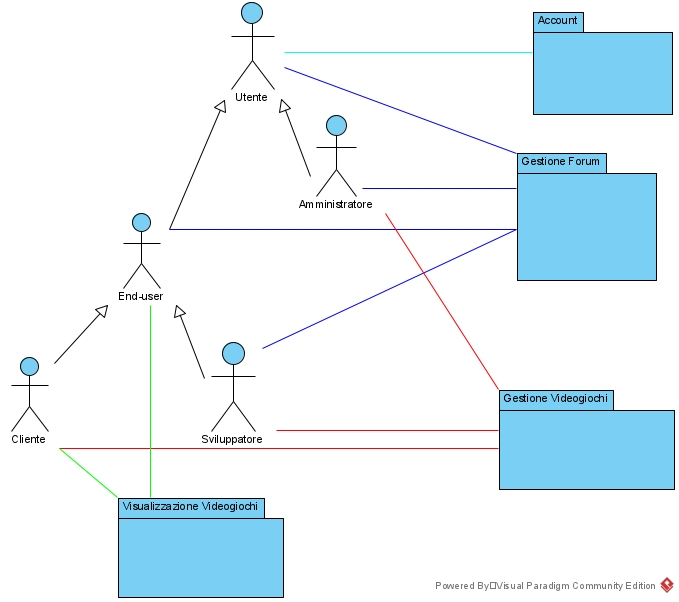
\includegraphics[width=\textwidth,height=\textheight,keepaspectratio]{Figure/UseCases/Generale.jpg}
\end{center}
\subsubsection{Account}
\begin{center}
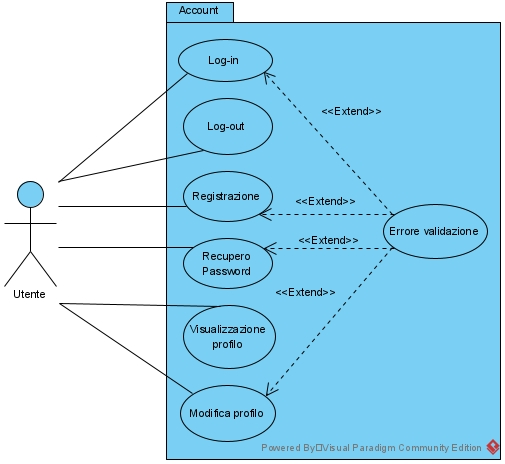
\includegraphics[width=\textwidth,height=\textheight,keepaspectratio]{Figure/UseCases/Account.jpg}
\end{center}

\newpage

\small\begin{tabular}{|| l | p{30em} ||} 
\hline
Nome & Log-in\\
\hline
Attori & Utente\\
\hline
Condizione d'ingresso & L’utente è registrato nel sistema e ha accesso alle sue credenziali\\
\hline
Flusso degli eventi &
	\begin{tabular}{p{14em}|p{14em}}
	\multicolumn{1}{c|}{\textbf{Utente}} & \multicolumn{1}{c}{\textbf{Sistema}} \\
	\hline
	L’utente accede alla pagina dedicata al log-in & \\
	\hline
	& Il sistema mostra un modulo per la richiesta dell’username e della password, entrambi come campi obbligatori \\
	\hline
	L’utente compila i dati necessari e li invia al sistema & \\
	\hline
	& Il sistema valida i dati lato client e lato server, procedendo all’autenticazione dell’utente \\
	\end{tabular}
\tabularnewline\hline
Condizione di uscita & La sessione dell’utente viene autenticata, permettendo l’accesso a funzionalità aggiuntive.\\
\hline
Eccezioni & Errore validazione client-side: uno dei campi è vuoto o non rispetta il pattern associato, all’utente viene mostrato il motivo del fallimento della trasmissione dei dati e viene nuovamente richiesto il suo input;
Errore validazione server-side: un dato dell’utente non rispetta il pattern richiesto o non è associato ad alcun account, quindi l’autenticazione fallisce e l’utente viene avvisato di aver inserito dati non corretti.\\
\hline
Requisiti Speciali & N/A\\
\hline
\end{tabular}

\newpage
\small\begin{tabular}{|| l | p{30em} ||} 
\hline
Nome & Log-out\\
\hline
Attori & Utente\\
\hline
Condizione d'ingresso & L’utente è attualmente autenticato\\
\hline
Flusso degli eventi &
	\begin{tabular}{p{14em}|p{14em}}
	\multicolumn{1}{c|}{\textbf{Utente}} & \multicolumn{1}{c}{\textbf{Sistema}} \\
	\hline
	L’utente decide di effettuare il log-out, cliccando sull’apposito pulsante & \\
	\hline
	& Il sistema invalida la sessione dell’utente, dando un messaggio di successo \\
	\end{tabular}
\tabularnewline\hline
Condizione di uscita & L’utente non ha più accesso alle funzionalità aggiuntive dedicate agli utenti autenticati\\
\hline
Eccezioni & N/A\\
\hline
Requisiti Speciali & N/A\\
\hline
\end{tabular}

\newpage
\small\begin{tabular}{|| l | p{30em} ||} 
\hline
Nome & Registrazione\\
\hline
Attori & Utente\\
\hline
Condizione d'ingresso & L’utente non è attualmente autenticato e non ha già un account all’interno del sistema\\
\hline
Flusso degli eventi &
	\begin{tabular}{p{14em}|p{14em}}
	\multicolumn{1}{c|}{\textbf{Utente}} & \multicolumn{1}{c}{\textbf{Sistema}} \\
	\hline
	L’utente non ancora registrato visualizza la schermata di registrazione & \\
	\hline
	& Il sistema mostra un modulo per la richiesta dei seguenti dati obbligatori: Username, E-mail, Password, Conferma password \\
	\hline
	L’utente compila i dati necessari e li invia al sistema & \\
	\hline
	& Il sistema valida i dati lato client e lato server, procedendo all’inserimento di un nuovo account nel caso di successo ed effettuando automaticamente il log-in. Inoltre, reindirizza l’utente alla pagina iniziale del sistema \\
	\end{tabular}
\tabularnewline\hline
Condizione di uscita & Viene generato un account nel database collegato alle credenziali fornite dall’utente, inoltre viene automaticamente autenticata la sessione dell’utente\\
\hline
Eccezioni & Errore validazione client-side: uno dei campi è vuoto o non rispetta il pattern associato, al visitatore viene mostrato il motivo del fallimento della trasmissione dei dati e viene nuovamente richiesto il suo input;
Errore validazione server-side: un dato dell’utente non rispetta il pattern richiesto o, nel caso di username o e-mail, esiste già all’interno del database. Viene comunicato l’errore all’utente e vengono nuovamente richiesti i dati necessari.\\
\hline
Requisiti Speciali & N/A\\
\hline
\end{tabular}

\newpage
\small\begin{tabular}{|| l | p{30em} ||} 
\hline
Nome & Recupero Password\\
\hline
Attori & Utente\\
\hline
Condizione d'ingresso & L’utente registrato non può ad effettuare il log-in, poiché ha dimenticato le credenziali associate al suo account.\\
\hline
Flusso degli eventi &
	\begin{tabular}{p{14em}|p{14em}}
	\multicolumn{1}{c|}{\textbf{Utente}} & \multicolumn{1}{c}{\textbf{Sistema}} \\
	\hline
	L’utente seleziona l’opzione “Ho dimenticato la password” & \\
	\hline
	& Il sistema chiede all’utente l’e-mail associata all’account al quale sta provando ad accedere \\
	\hline
	L’utente immette la sua e-mail & \\
	\hline
	& Il sistema valida l’e-mail lato client e lato server, trovando l’account associato, ed invia un link temporaneo all’email dell’account \\
	\hline
	L’utente naviga sul link ricevuto tramite e-mail & \\
	\hline
	& Il sistema chiede all’utente la nuova password da associare all’account, con le stesse regole di validazione della fase di registrazione, assieme ad un campo per confermarla \\
	\hline
	L’utente immette la nuova password & \\
	\hline
	& Il sistema applica la modifica al database ed effettua automaticamente il log-in dell’utente \\
	\end{tabular}
\tabularnewline\hline
Condizione di uscita & La password dell’utente viene aggiornata e l’utente viene automaticamente autenticato\\
\hline
Eccezioni & Errore validazione pattern: l’e-mail fornita non rispetta il pattern di una e-mail e viene chiesta nuovamente all’utente, oppure la password nuova non rispetta il formato richiesto e viene chiesta nuovamente all’utente.
Account associato non trovato: L’e-mail fornita non risulta associata ad alcun account e tale informazione viene comunicata all’utente, chiedendo nuovamente l’e-mail dell’account di cui resettare la password. \\
\hline
Requisiti Speciali & N/A\\
\hline
\end{tabular}

\newpage
\small\begin{tabular}{|| l | p{30em} ||} 
\hline
Nome & Visualizzazione Profilo\\
\hline
Attori & Utente\\
\hline
Condizione d'ingresso & L’utente è attualmente autenticato in una qualsiasi pagina del sistema\\
\hline
Flusso degli eventi &
	\begin{tabular}{p{14em}|p{14em}}
	\multicolumn{1}{c|}{\textbf{Utente}} & \multicolumn{1}{c}{\textbf{Sistema}} \\
	\hline
	L’utente clicca sul suo username nella barra di navigazione della pagina, scegliendo l’opzione “Visualizza profilo” & \\
	\hline
	& Il sistema visualizza dei dati dell’utente, ovvero username, e-mail, l’avatar ed il tipo dell’account (cliente, sviluppatore, amministratore), ma non la password per questioni di sicurezza. \\
	\end{tabular}
\tabularnewline\hline
Condizione di uscita & I dati del profilo dell’utente vengono mostrati all’utente stesso \\
\hline
Eccezioni & N/A\\
\hline
Requisiti Speciali & N/A\\
\hline
\end{tabular}

\newpage
\small\begin{tabular}{|| l | p{30em} ||} 
\hline
Nome & Modifica Profilo\\
\hline
Attori & Utente\\
\hline
Condizione d'ingresso & L’utente è autenticato ed è nella pagina di visualizzazione del suo profilo.\\
\hline
Flusso degli eventi &
	\begin{tabular}{p{14em}|p{14em}}
	\multicolumn{1}{c|}{\textbf{Utente}} & \multicolumn{1}{c}{\textbf{Sistema}} \\
	\hline
	L’utente clicca sul pulsante per abilitare la modifica delle sue informazioni. & \\
	\hline
	& Il sistema mostra un modulo contenente i campi per cambiare l’username, l’e-mail, l’avatar, la password e l’opzione per rendere il proprio account un account sviluppatore. \\
	\hline
	L’utente inserisce i dati da cambiare, assieme alla sua password attuale. & \\
	\hline
	& Il sistema valida i dati inseriti dall’utente con gli stessi pattern usati in fase di registrazione, controllando inoltre che la password inserita sia corretta. In caso di successo, i dati dell’account vengono aggiornati e l’utente viene rimandato alla pagina di visualizzazione del proprio profilo \\
	\end{tabular}
\tabularnewline\hline
Condizione di uscita & I dati dell’utente vengono modificati con successo. Nel caso l’utente abbia selezionato l’opzione sviluppatore, diventa uno sviluppatore.\\
\hline
Eccezioni & Errore validazione: Vengono richiesti nuovamente i dati all’utente, indicando il motivo per cui sono stati rifiutati.\\
\hline
Requisiti Speciali & N/A\\
\hline
\end{tabular}

\subsubsection{Visualizzazione Videogiochi}
\begin{center}
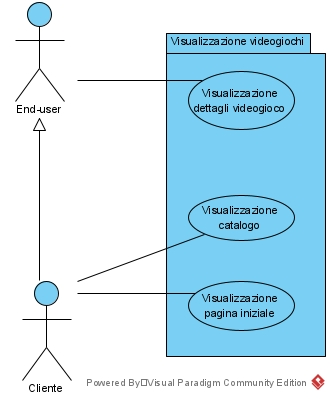
\includegraphics[width=\textwidth,height=\textheight,keepaspectratio]{Figure/UseCases/VisualizzazioneVideogioco.jpg}
\end{center}

\newpage
\small\begin{tabular}{|| l | p{30em} ||} 
\hline
Nome & Visualizzazione Dettagli Videogioco\\
\hline
Attori & End-user\\
\hline
Condizione d'ingresso & L’end-user naviga sulla pagina dedicata al videogioco dal catalogo o direttamente tramite URL\\
\hline
Flusso degli eventi &
	\begin{tabular}{p{14em}|p{14em}}
	\multicolumn{1}{c|}{\textbf{Utente}} & \multicolumn{1}{c}{\textbf{Sistema}} \\
	\hline
	& Il sistema fornisce i dettagli del videogioco selezionato, ovvero logo, titolo, delle immagini d’esempio (massimo 3), la descrizione estesa del videogioco, i tags ed il prezzo, quest’ultimo come testo di un pulsante che permette l’acquisto o l’installazione. In una sezione separata, vengono mostrate le recensioni degli utenti, inoltre in una sezione immediatamente visibile viene mostrato un pulsante che rimanda al forum dedicato al videogioco. \\
	\end{tabular}
\tabularnewline\hline
Condizione di uscita & Tutte le informazioni relative al videogioco inserite nel sistema vengono mostrate all’end-user.\\
\hline
Eccezioni & N/A\\
\hline
Requisiti Speciali & N/A\\
\hline
\end{tabular}

\newpage
\small\begin{tabular}{|| l | p{30em} ||} 
\hline
Nome & Visualizzazione Catalogo\\
\hline
Attori & Cliente\\
\hline
Condizione d'ingresso & Il cliente naviga sulla pagina dedicata al catalogo\\
\hline
Flusso degli eventi &
	\begin{tabular}{p{14em}|p{14em}}
	\multicolumn{1}{c|}{\textbf{Utente}} & \multicolumn{1}{c}{\textbf{Sistema}} \\
	\hline
	& Il sistema fornisce un listino di prodotti, categorizzati tramite le informazioni essenziali (logo, titolo, parte iniziale della descrizione, prezzo e tags) \\
	\hline
	Il cliente, tramite una sezione dedicata all’interno della stessa pagina, può filtrare i contenuti secondo vari tipi di criteri: titolo (similarità), prezzo (intervallo), tags (in due modi distinti: tag obbligatorie, le quali devono essere tutte possedute dal gioco, e tag opzionali, per le quali basta che una sia presente per rendere il gioco valido per il filtro) e acquistato (se il gioco è presente nella libreria dell’utente o no). Il cliente può anche decidere l’ordine di visualizzazione dei videogiochi (per prezzo crescente o decrescente) & \\
	\hline
	& Il sistema filtra tutti i videogiochi presenti in quel momento all’interno del sistema secondo i criteri forniti dal cliente, visualizzando solo i videogiochi validi per tali criteri, con l’ordinamento fornito dall’utente o in ordine decrescente di prezzo se non indicato, se esistono, altrimenti al cliente viene notificata l’assenza di videogiochi che rispettano il set di criteri forniti \\
	\end{tabular}
\tabularnewline\hline
Condizione di uscita & L’utente visualizza i videogiochi filtrati e ordinati secondo i criteri forniti dall’utente\\
\hline
Eccezioni & N/A\\
\hline
Requisiti Speciali & N/A\\
\hline
\end{tabular}

\newpage
\small\begin{tabular}{|| l | p{30em} ||} 
\hline
Nome & Visualizzazione Pagina Iniziale\\
\hline
Attori & Cliente\\
\hline
Condizione d'ingresso & Il cliente naviga sulla pagina iniziale del sistema\\
\hline
Flusso degli eventi &
	\begin{tabular}{p{14em}|p{14em}}
	\multicolumn{1}{c|}{\textbf{Utente}} & \multicolumn{1}{c}{\textbf{Sistema}} \\
	\hline
	& Il sistema mostra una serie di raccolte di dieci giochi ciascuna: i giochi attualmente sponsorizzati dalla piattaforma, i giochi con più download e gli ultimi giochi pubblicati sulla piattaforma. Se il cliente è autenticato, viene mostrata una ulteriore raccolta con dei giochi consigliati in base alla similarità tra i tags dei giochi acquistati valutati positivamente e tutti quelli presenti in piattaforma, mostrando per primi i giochi con più tags in comune.
	Per ogni gioco viene mostrato il titolo, il prezzo e le tags. \\
	\end{tabular}
\tabularnewline\hline
Condizione di uscita & L’utente ha una visione iniziale del sistema e una possibile selezione di giochi a cui prestare attenzione.\\
\hline
Eccezioni & N/A\\
\hline
Requisiti Speciali & N/A\\
\hline
\end{tabular}

\subsubsection{Gestione Videogiochi}
\begin{center}
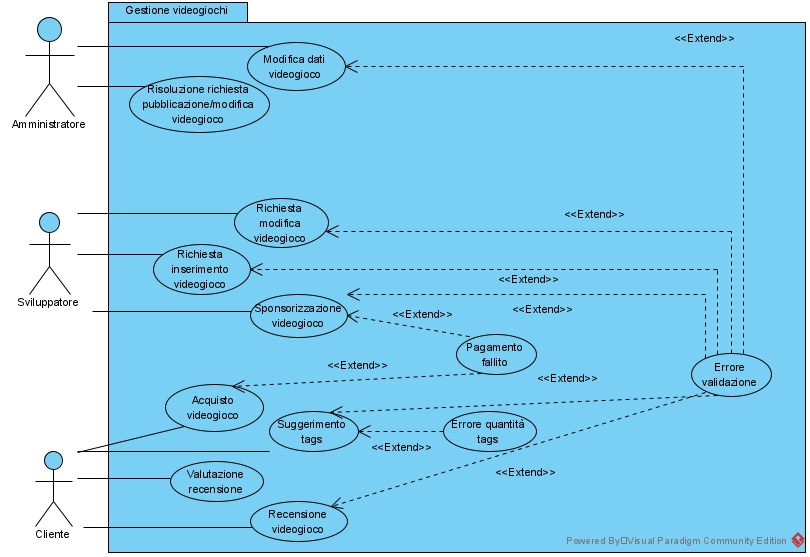
\includegraphics[width=\textwidth,height=\textheight,keepaspectratio]{Figure/UseCases/Videogioco.jpg}
\end{center}

\newpage
\small\begin{tabular}{|| l | p{30em} ||} 
\hline
Nome & Modifica Dati Videogioco\\
\hline
Attori & Amministratore\\
\hline
Condizione d'ingresso & L’amministratore è autenticato ed è sulla pagina dei dettagli di un videogioco\\
\hline
Flusso degli eventi &
	\begin{tabular}{p{14em}|p{14em}}
	\multicolumn{1}{c|}{\textbf{Utente}} & \multicolumn{1}{c}{\textbf{Sistema}} \\
	\hline
	L’amministratore avvia la modifica dei dettagli del videogioco tramite l’apposito pulsante & \\
	\hline
	& Il sistema mostra un modulo simile a quello offerto agli sviluppatori, con l’opzione aggiuntiva di poter modificare l’autore stesso del videogioco \\
	\hline
	L’utente applica le modifiche necessarie. & \\
	\hline
	& Il sistema applica immediatamente le modifiche richieste dall’utente, senza creare una richiesta di modifica. \\
	\end{tabular}
\tabularnewline\hline
Condizione di uscita & Le modifiche richieste vengono applicate immediatamente \\
\hline
Eccezioni & Errore validazione: Vengono richiesti nuovamente i dati all’utente, indicando il motivo per cui sono stati rifiutati.\\
\hline
Requisiti Speciali & N/A\\
\hline
\end{tabular}

\newpage
\small\begin{tabular}{|| l | p{30em} ||} 
\hline
Nome & Risoluzione richiesta pubblicazione o modifica videogioco\\
\hline
Attori & Amministratore\\
\hline
Condizione d'ingresso & L’amministratore è autenticato ed è sul pannello amministrativo del sistema.\\
\hline
Flusso degli eventi &
	\begin{tabular}{p{14em}|p{14em}}
	\multicolumn{1}{c|}{\textbf{Utente}} & \multicolumn{1}{c}{\textbf{Sistema}} \\
	\hline
	L’amministratore visualizza la coda di richieste in ordine cronologico crescente e seleziona una richiesta per processarla & \\
	\hline
	& Il sistema mostra i dati compilati dallo sviluppatore, assieme all’autore della richiesta (lo sviluppatore stesso) \\
	\hline
	L’amministratore revisiona i dati inseriti ed esegue una serie di test sull’eseguibile fornito, per assicurarsi che non sia malevolo, per poi decidere di approvare o respingere la richiesta, specificando un eventuale commento nel caso sia necessario. & \\
	\hline
	& Il sistema segna la richiesta come processata ed applica le modifiche richieste, nel caso la richiesta sia stata approvata. Inoltre, manda una e-mail all’autore della richiesta contenente l’esito scelto dall’amministratore ed il suo commento.\\
	\end{tabular}
\tabularnewline\hline
Condizione di uscita & La richiesta viene processata con successo e viene nascosta nella coda visibile agli amministratori, ma viene mantenuta nel database per poterla visionare in caso ci fosse il bisogno.\\
\hline
Eccezioni & N/A\\
\hline
Requisiti Speciali & N/A\\
\hline
\end{tabular}

\newpage
\small\begin{tabular}{|| l | p{30em} ||} 
\hline
Nome & Richiesta modifica dati videogioco\\
\hline
Attori & Sviluppatore\\
\hline
Condizione d'ingresso & Lo sviluppatore è autenticato ed è sulla pagina dei dettagli di un videogioco di cui lui è l’autore.\\
\hline
Flusso degli eventi &
	\begin{tabular}{p{14em}|p{14em}}
	\multicolumn{1}{c|}{\textbf{Utente}} & \multicolumn{1}{c}{\textbf{Sistema}} \\
	\hline
	Lo sviluppatore clicca sul pulsante per iniziare la modifica dei dati del suo videogioco. & \\
	\hline
	& Il sistema mostra un modulo uguale a quello usato per la richiesta di pubblicazione di un videogioco, con i campi aventi i valori attualmente salvati nel sistema per il videogioco scelto. Viene inoltre mostrato un campo addizionale per la pubblicazione di un aggiornamento del proprio videogioco, il quale richiede l’eseguibile e un commento che descrive i cambiamenti, con un massimo di mille caratteri. \\
	\hline
	Lo sviluppatore modifica i dati secondo le sue preferenze. & \\
	\hline
	& Il sistema valida le modifiche secondo gli stessi criteri della richiesta di pubblicazione di un videogioco. In caso di successo, la richiesta di modifica dei dati viene inserita in una coda visualizzabile dagli amministratori. L’utente viene rimandato sulla pagina dei dettagli del suo videogioco, con un simbolo indicante che la sua richiesta è attualmente da processare. \\
	\end{tabular}
\tabularnewline\hline
Condizione di uscita & La richiesta di modifica viene inserita in una coda visualizzabile dagli amministratori. In caso di approvazione, le modifiche richieste vengono applicate.\\
\hline
Eccezioni & Errore validazione: Vengono richiesti nuovamente i dati all’utente, indicando il motivo per cui sono stati rifiutati.\\
\hline
Requisiti Speciali & N/A\\
\hline
\end{tabular}

\newpage
\small\begin{tabular}{|| l | p{30em} ||} 
\hline
Nome & Richiesta Pubblicazione Videogioco\\
\hline
Attori & Sviluppatore\\
\hline
Condizione d'ingresso & Lo sviluppatore è autenticato, è in una qualsiasi pagina del sistema ed è intenzionato a pubblicare un suo videogioco.\\
\hline
Flusso degli eventi &
	\begin{tabular}{p{14em}|p{14em}}
	\multicolumn{1}{c|}{\textbf{Utente}} & \multicolumn{1}{c}{\textbf{Sistema}} \\
	\hline
	Lo sviluppatore seleziona l’opzione “Pubblica il tuo videogioco” & \\
	\hline
	& Il sistema mostra un modulo allo sviluppatore, chiedendo i dati del gioco quali titolo, descrizione, prezzo, logo e massimo tre immagini riassuntive \\
	\hline
	Lo sviluppatore compila le informazioni necessarie & \\
	\hline
	& Il sistema valida i campi, controllando se il titolo è composto da massimo 30 caratteri, se la descrizione è composta da massimo 5000 caratteri, se il logo è un numero reale con massimo due cifre dopo la virgola e se le immagini ed il logo siano di massimo 5MB l’una. In caso di successo, viene mostrato un ulteriore modulo per permettere il caricamento dell’eseguibile del videogioco \\
	\hline
	Lo sviluppatore carica l’eseguibile del proprio videogioco. & \\
	\hline
	& Il sistema salva le informazioni nel database, rimandando l’utente ad una pagina di successo indicando che la sua richiesta verrà processata dagli amministratori nel minor tempo possibile. \\
	\end{tabular}
\tabularnewline\hline
Condizione di uscita & La richiesta dello sviluppatore viene inserita nella coda visibile dagli amministratori, in attesa di approvazione.\\
\hline
Eccezioni & Errore validazione: Vengono richiesti nuovamente i dati all’utente, indicando il motivo per cui sono stati rifiutati.\\
\hline
Requisiti Speciali & N/A\\
\hline
\end{tabular}

\newpage
\small\begin{tabular}{|| l | p{30em} ||} 
\hline
Nome & Sponsorizzazione Videogioco\\
\hline
Attori & Sviluppatore\\
\hline
Condizione d'ingresso & Lo sviluppatore è autenticato ed è sulla pagina dei dettagli di un videogioco di cui lui è l’autore.\\
\hline
Flusso degli eventi &
	\begin{tabular}{p{14em}|p{14em}}
	\multicolumn{1}{c|}{\textbf{Utente}} & \multicolumn{1}{c}{\textbf{Sistema}} \\
	\hline
	Lo sviluppatore clicca sul pulsante per iniziare il processo di sponsorizzazione del suo videogioco. & \\
	\hline
	& Il sistema richiede allo sviluppatore le settimane in cui deve valere la sponsorizzazione, mostrando come opzioni solo le settimane non aventi già più di dieci sponsorizzazioni fissate \\
	\hline
	Lo sviluppatore seleziona le settimane che preferisce. & \\
	\hline
	& Il sistema, in tempo reale, mostra la variazione del costo in base alle settimane selezionate dall’utente \\
	\hline
	Lo sviluppatore procede con il pagamento tramite un servizio esterno dedicato. & \\
	\hline
	& Il sistema riceve l’OK dal servizio esterno e assegna le settimane selezionate al videogioco scelto \\
	\end{tabular}
\tabularnewline\hline
Condizione di uscita & Il videogioco comparirà nella pagina iniziale del sistema durante le settimane selezionate, nella raccolta apposita.\\
\hline
Eccezioni & Errore validazione data: Vengono richiesti nuovamente i dati all’utente, indicando il motivo per cui sono stati rifiutati (settimana non disponibile).
Errore pagamento: il servizio esterno non dà l’OK per il pagamento eseguito e il sistema chiede all’utente di riprovare. \\
\hline
Requisiti Speciali & È necessario un servizio esterno per gestire il pagamento, come ad esempio Stripe.\\
\hline
\end{tabular}

\newpage
\small\begin{tabular}{|| l | p{30em} ||} 
\hline
Nome & Acquisto Videogioco\\
\hline
Attori & Cliente\\
\hline
Condizione d'ingresso & Il cliente è autenticato ed è sulla pagina dei dettagli di uno specifico videogioco\\
\hline
Flusso degli eventi &
	\begin{tabular}{p{14em}|p{14em}}
	\multicolumn{1}{c|}{\textbf{Utente}} & \multicolumn{1}{c}{\textbf{Sistema}} \\
	\hline
	Il cliente clicca sul pulsante per avviare la procedura di acquisto di un videogioco. & \\
	\hline
	& Il sistema processa il pagamento se necessario e, nel caso vada a buon fine o se il gioco è gratuito, aggiunge il videogioco nella libreria del cliente e procede a rendere disponibile l’eseguibile al cliente \\
	\hline
	Il cliente sceglie la versione che vuole e procede con il download & \\
	\hline
	& Il sistema mostra tutte le versioni del videogioco attualmente presenti nella piattaforma, assieme al changelog relativo ad ogni versione \\
	\hline
	L’utente installa la versione scelta del videogioco con successo & \\
	\end{tabular}
\tabularnewline\hline
Condizione di uscita & Il videogioco scelto viene inserito nella libreria del cliente, ciò implica che il cliente può anche scrivere una recensione per tale videogioco, votare le recensioni esistenti per quel videogioco e partecipare in modalità di scrittura al forum dedicato.\\
\hline
Eccezioni & Pagamento Fallito: Il cliente rifiuta di pagare o il servizio esterno che gestisce il pagamento riporta un errore. Tale errore viene mostrato all’utente.\\
\hline
Requisiti Speciali & Si assume che il dispositivo sia compatibile con il gioco che l’utente sta provando ad installare.
È necessario un servizio esterno per gestire il pagamento, come ad esempio Stripe.\\
\hline
\end{tabular}

\newpage
\small\begin{tabular}{|| l | p{30em} ||} 
\hline
Nome & Suggerimento Tags\\
\hline
Attori & Cliente\\
\hline
Condizione d'ingresso & Il cliente è autenticato ed è attualmente nella schermata di visualizzazione dei dettagli di un videogioco che ha acquistato.\\
\hline
Flusso degli eventi &
	\begin{tabular}{p{14em}|p{14em}}
	\multicolumn{1}{c|}{\textbf{Utente}} & \multicolumn{1}{c}{\textbf{Sistema}} \\
	\hline
	Il cliente sceglie l’opzione per l’aggiunta di una nuova tag relativa al videogioco in analisi & \\
	\hline
	& Il sistema presenta al cliente una schermata composta da un elenco delle 20 tag attualmente più popolari, un elenco delle tag attualmente suggerite dall’utente stesso e un campo testuale per l’aggiunta di una nuova tag \\
	\hline
	Il cliente sceglie se consigliare una o più tag attualmente popolari, o se consigliarne una non presente nell’elenco, od entrambe & \\
	\hline
	& Il sistema provvede, in ogni caso, ad aggiungere nel database una corrispondenza tra il cliente, il videogioco e la tag suggerita. Nel caso di una nuova tag, il testo fornito dal cliente viene validato per controllare che non superi i venti caratteri. Nel caso il cliente provi a suggerire più di cinque tags, il sistema respinge la richiesta del cliente \\
	\hline
	Il cliente può, inoltre, rimuovere un suggerimento già fatto cliccando sulla tag da rimuovere dall’elenco dei suoi suggerimenti & \\
	\hline
	& Il sistema rimuove correttamente il suggerimento dal sistema \\
	\end{tabular}
\tabularnewline\hline
Condizione di uscita & Il suggerimento della tag relativa al videogioco in analisi viene inserito nel database del sistema. Nel caso la tag diventa tra le dieci più popolari, viene anche mostrata nella pagina dei dettagli del videogioco.\\
\hline
Eccezioni & Errore validazione: La tag suggerita dall’utente è troppo lunga, viene quindi mostrato nuovamente il campo testuale segnalando tale errore.
Errore quantità tag: Il cliente ha suggerito già cinque tag, quindi viene rimandato al modulo segnalando l’errore e consigliando la rimozione di una tag suggerita per continuare. \\
\hline
Requisiti Speciali & N/A\\
\hline
\end{tabular}

\newpage
\small\begin{tabular}{|| l | p{30em} ||} 
\hline
Nome & Valutazione di una Recensione\\
\hline
Attori & Cliente\\
\hline
Condizione d'ingresso & Il cliente è autenticato ed è attualmente nella schermata di visualizzazione dei dettagli di un videogioco da lui acquistato, nella sezione dedicata alle recensioni, con il focus su una recensione che non ha ancora valutato.\\
\hline
Flusso degli eventi &
	\begin{tabular}{p{14em}|p{14em}}
	\multicolumn{1}{c|}{\textbf{Utente}} & \multicolumn{1}{c}{\textbf{Sistema}} \\
	\hline
	Il cliente visualizza le recensioni del videogioco e ha la possibilità, attraverso due pulsanti appositi, di valutare positivamente o negativamente la recensione, scegliendone uno& \\
	\hline
	& Il sistema salva la valutazione del cliente, per non permettere una seconda valutazione in futuro alla stessa recensione \\
	\hline
	Il cliente visualizzerà il pulsante da lui cliccato con uno stile indicante che è stato cliccato da lui, ogni volta che andrà a vedere quella particolare recensione valutata & \\
	\end{tabular}
\tabularnewline\hline
Condizione di uscita & La valutazione della recensione viene salvata nel database.\\
\hline
Eccezioni & N/A\\
\hline
Requisiti Speciali & N/A\\
\hline
\end{tabular}

\newpage
\small\begin{tabular}{|| l | p{30em} ||} 
\hline
Nome & Recensione di un Videogioco\\
\hline
Attori & Cliente\\
\hline
Condizione d'ingresso & Il cliente è autenticato ed è sulla pagina dei dettagli di un videogioco presente nella sua libreria. Inoltre, l’utente non deve avere già recensito il videogioco.\\
\hline
Flusso degli eventi &
	\begin{tabular}{p{14em}|p{14em}}
	\multicolumn{1}{c|}{\textbf{Utente}} & \multicolumn{1}{c}{\textbf{Sistema}} \\
	\hline
	Il cliente utilizza il modulo nella sezione delle recensioni per dare il suo giudizio al videogioco, indicando se il giudizio è positivo o no e commentando la sua motivazione & \\
	\hline
	& Il sistema valida i dati lato client e lato server, controllando che il giudizio sia un valore booleano e che il commento non superi i 5000 caratteri. In caso di successo, inserisce la recensione nel database \\
	\end{tabular}
\tabularnewline\hline
Condizione di uscita & La recensione del videogioco viene inserita correttamente nel database.\\
\hline
Eccezioni & Errore validazione: Vengono richiesti nuovamente i dati all’utente, indicando il motivo per cui sono stati rifiutati.\\
\hline
Requisiti Speciali & N/A\\
\hline
\end{tabular}

\subsubsection{Gestione Forum}
\begin{center}
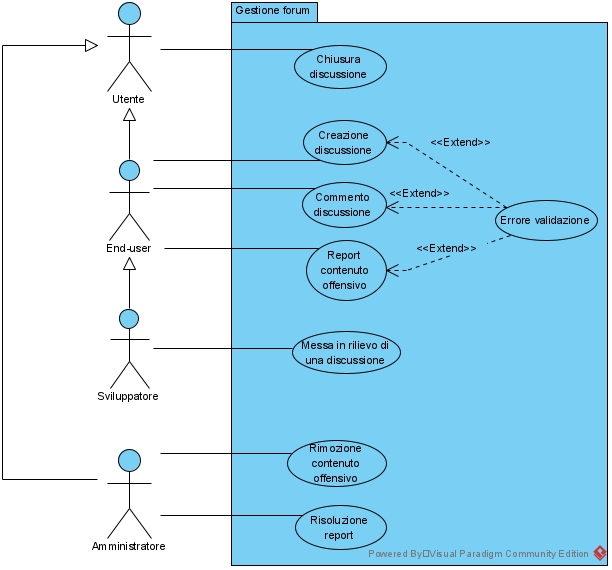
\includegraphics[width=\textwidth,height=\textheight,keepaspectratio]{Figure/UseCases/Forum.jpg}
\end{center}

\newpage
\small\begin{tabular}{|| l | p{30em} ||} 
\hline
Nome & Chiusura di una Discussione\\
\hline
Attori & Utente\\
\hline
Condizione d'ingresso & L’utente deve essere l’autore della discussione da chiudere, se è un cliente. Se è uno sviluppatore, deve essere l’autore del videogioco del forum contenente la discussione. Gli amministratori possono chiudere qualsiasi discussione.
L’utente è sulla pagina contenente la discussione. \\
\hline
Flusso degli eventi &
	\begin{tabular}{p{14em}|p{14em}}
	\multicolumn{1}{c|}{\textbf{Utente}} & \multicolumn{1}{c}{\textbf{Sistema}} \\
	\hline
	L’utente, guardando il commento iniziale della discussione, clicca sul pulsante per chiudere la discussione & \\
	\hline
	& Il sistema provvede a chiudere la discussione, non permettendo la creazione di altri commenti \\
	\end{tabular}
\tabularnewline\hline
Condizione di uscita & La discussione diventa di sola lettura\\
\hline
Eccezioni & N/A\\
\hline
Requisiti Speciali & N/A\\
\hline
\end{tabular}

\newpage
\small\begin{tabular}{|| l | p{30em} ||} 
\hline
Nome & Creazione di una Discussione\\
\hline
Attori & End-user\\
\hline
Condizione d'ingresso & L’end-user è autenticato ed è sul forum di un videogioco presente nella sua libreria.\\
\hline
Flusso degli eventi &
	\begin{tabular}{p{14em}|p{14em}}
	\multicolumn{1}{c|}{\textbf{Utente}} & \multicolumn{1}{c}{\textbf{Sistema}} \\
	\hline
	L’end-user visualizza tutte le discussioni attualmente esistenti in un formato a griglia, dalla più recente alla meno. Le prime discussioni visualizzate sono quelle messe in rilievo dagli sviluppatori del videogioco interessato. L'end-user procede a cliccare sul pulsante per la creazione di una nuova discussione. & \\
	\hline
	& Il sistema mostra un modulo all’end-user, richiedendo il titolo della discussione e il corpo del messaggio iniziale \\
	\hline
	L’end-user compila i dati necessari & \\
	\hline
	& Il sistema valida i dati, controllando se il titolo è composto da massimo 100 caratteri e se il corpo è di massimo 1000 caratteri. In caso di successo, inserisce la nuova discussione nel database \\
	\end{tabular}
\tabularnewline\hline
Condizione di uscita & La discussione viene salvata nel database e mostrata come prima dopo le discussioni poste in rilievo, poiché è la più recente.\\
\hline
Eccezioni & Errore validazione: Vengono richiesti nuovamente i dati all’utente, indicando il motivo per cui sono stati rifiutati.\\
\hline
Requisiti Speciali & N/A\\
\hline
\end{tabular}

\newpage
\small\begin{tabular}{|| l | p{30em} ||} 
\hline
Nome & Commento di una Discussione\\
\hline
Attori & End-user\\
\hline
Condizione d'ingresso & L’end-user è autenticato ed è sul forum di un videogioco presente nella sua libreria.\\
\hline
Flusso degli eventi &
	\begin{tabular}{p{14em}|p{14em}}
	\multicolumn{1}{c|}{\textbf{Utente}} & \multicolumn{1}{c}{\textbf{Sistema}} \\
	\hline
	L’end-user sceglie una discussione tra quelle visualizzate nella griglia principale & \\
	\hline
	& Il sistema mostra il messaggio iniziale della discussione, assieme a tutti i commenti attualmente esistenti per quella discussione in ordine cronologico, assieme ad un modulo per commentare la discussione dove viene richiesto il corpo del messaggio \\
	\hline
	L’end-user compila il modulo con il suo commento & \\
	\hline
	& Il sistema valida il commento, controllando se è composto da massimo mille caratteri. In caso di successo, aggiunge il commento al database collegandolo alla discussione relativa \\
	\end{tabular}
\tabularnewline\hline
Condizione di uscita & Il commento dell’end-user viene salvato nel database.\\
\hline
Eccezioni & Errore validazione: Vengono richiesti nuovamente i dati all’utente, indicando il motivo per cui sono stati rifiutati.\\
\hline
Requisiti Speciali & N/A\\
\hline
\end{tabular}

\newpage
\small\begin{tabular}{|| l | p{30em} ||} 
\hline
Nome & Report Contenuto Offensivo\\
\hline
Attori & End-user\\
\hline
Condizione d'ingresso & L’end-user è autenticato ed è sulla pagina dei dettagli di un videogioco, oppure in una discussione di un videogioco.\\
\hline
Flusso degli eventi &
	\begin{tabular}{p{14em}|p{14em}}
	\multicolumn{1}{c|}{\textbf{Utente}} & \multicolumn{1}{c}{\textbf{Sistema}} \\
	\hline
	L’end-user segnala del contenuto offensivo tramite un apposito pulsante posto su ogni contenuto (recensione oppure commento di una discussione) & \\
	\hline
	& Il sistema mostra un pop-up all’end-user, chiedendo la motivazione per il quale si vuole generare un report \\
	\hline
	L’end-user commenta il motivo & \\
	\hline
	& Il sistema valida la motivazione controllando se è formata da meno di cento caratteri. Nel caso lo sia, genera un nuovo report con l’end-user come autore, con la motivazione fornita e con una corrispondenza al contenuto segnalato, assieme ad uno stato iniziale di “Non processato” \\
	\end{tabular}
\tabularnewline\hline
Condizione di uscita & Il report viene salvato nel database e viene mostrato in una coda visibile agli amministratori del sistema come report da processare.\\
\hline
Eccezioni & Errore validazione: Viene richiesto all’end-user la motivazione, segnalando che deve essere composta da meno di cento caratteri.\\
\hline
Requisiti Speciali & N/A\\
\hline
\end{tabular}

\newpage
\small\begin{tabular}{|| l | p{30em} ||} 
\hline
Nome & Messa in rilievo di una discussione\\
\hline
Attori & Sviluppatore\\
\hline
Condizione d'ingresso & Lo sviluppatore è autenticato ed è sul forum di un videogioco di cui lui è l’autore.\\
\hline
Flusso degli eventi &
	\begin{tabular}{p{14em}|p{14em}}
	\multicolumn{1}{c|}{\textbf{Utente}} & \multicolumn{1}{c}{\textbf{Sistema}} \\
	\hline
	Lo sviluppatore seleziona le discussioni da porre in rilievo, per poi cliccare il pulsante apposito & \\
	\hline
	& Il sistema pone le discussioni selezionate in rilievo, in ordine cronologico decrescente, prima di ogni altra discussione \\
	\end{tabular}
\tabularnewline\hline
Condizione di uscita & Le discussioni selezionate sono immediatamente visibili ai visualizzatori del forum.\\
\hline
Eccezioni & N/A\\
\hline
Requisiti Speciali & N/A\\
\hline
\end{tabular}

\newpage
\small\begin{tabular}{|| l | p{30em} ||} 
\hline
Nome & Rimozione di un contenuto offensivo\\
\hline
Attori & Amministratore\\
\hline
Condizione d'ingresso & L’amministratore è autenticato ed è su una discussione o su una pagina di dettagli di un videogioco contenente il contenuto offensivo da rimuovere.\\
\hline
Flusso degli eventi &
	\begin{tabular}{p{14em}|p{14em}}
	\multicolumn{1}{c|}{\textbf{Utente}} & \multicolumn{1}{c}{\textbf{Sistema}} \\
	\hline
	L’amministratore sceglie l’opzione per nascondere il contenuto offensivo & \\
	\hline
	& Il sistema mantiene nel database il contenuto offensivo ma lo segna come nascosto.
	Il commento viene nascosto a tutti gli utenti non amministratori e che non corrispondono all’autore del commento \\	
	\end{tabular}
\tabularnewline\hline
Condizione di uscita & Il commento viene segnato come nascosto.\\
\hline
Eccezioni & N/A\\
\hline
Requisiti Speciali & N/A\\
\hline
\end{tabular}

\newpage
\small\begin{tabular}{|| l | p{30em} ||} 
\hline
Nome & Risoluzione di un Report\\
\hline
Attori & Amministratore\\
\hline
Condizione d'ingresso & L’amministratore è autenticato ed è sul pannello amministrativo del sistema.\\
\hline
Flusso degli eventi &
	\begin{tabular}{p{14em}|p{14em}}
	\multicolumn{1}{c|}{\textbf{Utente}} & \multicolumn{1}{c}{\textbf{Sistema}} \\
	\hline
	L’amministratore visualizza la lista di report raggruppati secondo il contenuto segnalato e ordinati per numero di report associati al singolo contenuto. Ogni report è associato al link del contenuto segnalato, assieme a due pulsanti per accettare o rifiutare il report. & \\
	\hline
	L’utente clicca sul contenuto e decide se rimuoverlo seguendo i passaggi del caso d’uso “Rimozione di un contenuto offensivo” & \\
	\hline
	L’utente torna nel pannello amministrativo del sistema e clicca sul pulsante per accettare o rifiutare il report & \\
	\hline
	& Il sistema marca il report come processato, segnalando a tutti gli autori dei report associati al contenuto la risoluzione positiva o negativa di esso \\
	\end{tabular}
\tabularnewline\hline
Condizione di uscita & I report vengono processati.\\
\hline
Eccezioni & N/A\\
\hline
Requisiti Speciali & N/A\\
\hline
\end{tabular}

\newpage
\subsection{Modello ad oggetti}
\subsubsection{Diagramma delle classi}
Il primo diagramma delle entità rappresenta entità e associazioni con un focus sull’entità Videogioco.
\begin{center}
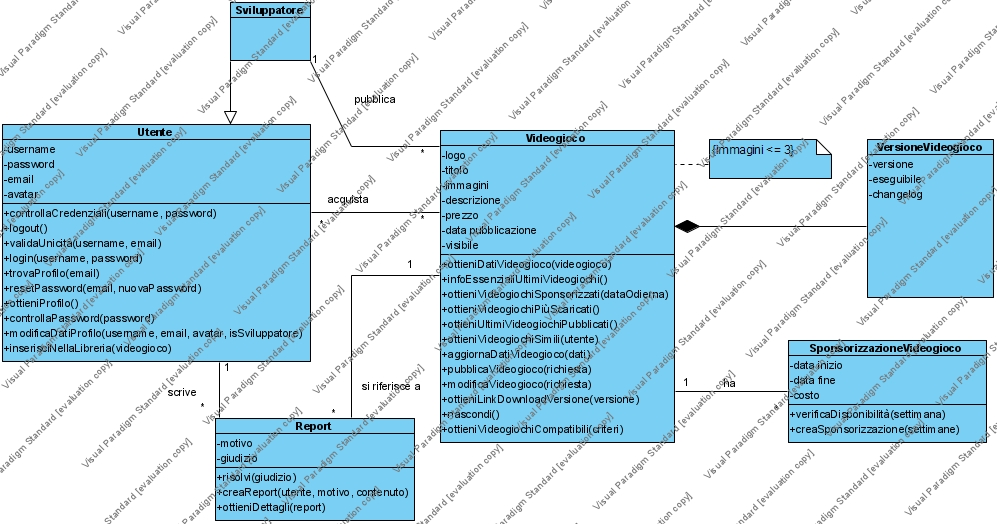
\includegraphics[width=\textwidth,height=\textheight,keepaspectratio]{Figure/ClassDiagrams/FocusVideogioco.jpg}
\end{center}

Il secondo diagramma rappresenta entità e associazioni con un focus sull’utente.
\begin{center}
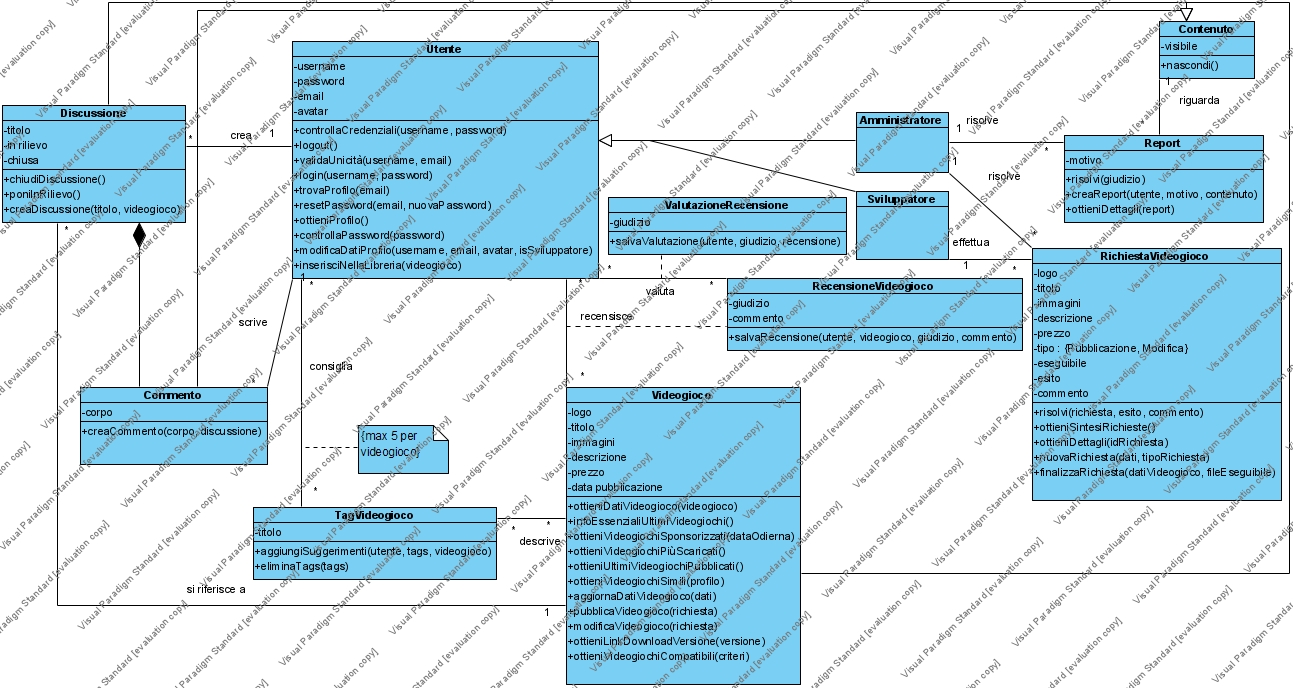
\includegraphics[width=\textwidth,height=\textheight,keepaspectratio]{Figure/ClassDiagrams/FocusUtente.jpg}
\end{center}

\newpage
\small\begin{tabular}{|| l | p{25em} ||}
\multicolumn{1}{||c|}{\textbf{Entità}} & \multicolumn{1}{c||}{\textbf{Descrizione}} \\
\hline
Utente & Descrive un profilo di un singolo utente all’interno del sistema, con determinati attributi forniti in fase di registrazione.\\
\hline
Sviluppatore & Descrive un particolare tipo di Utente che può pubblicare videogiochi.\\
\hline
Amministratore & Descrive un particolare tipo di Utente che può risolvere report e gestire il sistema.\\
\hline
Videogioco & È il prodotto principale offerto dal sistema ai clienti.\\
\hline
VersioneVideogioco & Rappresenta un singolo contenuto scaricabile di un determinato videogioco.\\
\hline
Recensione & Una valutazione da parte di un utente per un particolare videogioco.\\
\hline
TagVideogioco & Una caratteristica che sintetizza una caratteristica di un videogioco.\\
\hline
RichiestaVideogioco & Descrive una richiesta relativa ad un videogioco, fornita da uno Sviluppatore, per eseguire una modifica nel sistema.\\
\hline
RichiestaPubblicazioneVideogioco & Un particolare tipo di RichiestaVideogioco, che descrive l’azione di pubblicazione di esso.\\
\hline
RichiestaModificaVideogioco & Un particolare tipo di RichiestaVideogioco, che descrive l’azione di modifica dei dati di esso.\\
\hline
SponsorizzazioneVideogioco & Un servizio pagato da uno sviluppatore per porre in prima pagina il proprio videogioco.\\
\hline
Discussione & L’inizio di una conversazione su un forum dedicato ad un videogioco da parte degli utenti registrati nel sistema.\\
\hline
Commento & Un singolo messaggio all’interno di una discussione da parte di un utente.\\
\hline
Report & Una segnalazione da parte di un utente con l’obiettivo di rimuovere un contenuto offensivo.\\
\hline
\end{tabular}

\newpage
\subsection{Modello dinamico}
\subsubsection{Diagrammi di sequenza}
\paragraph{Log-in}
\begin{center}
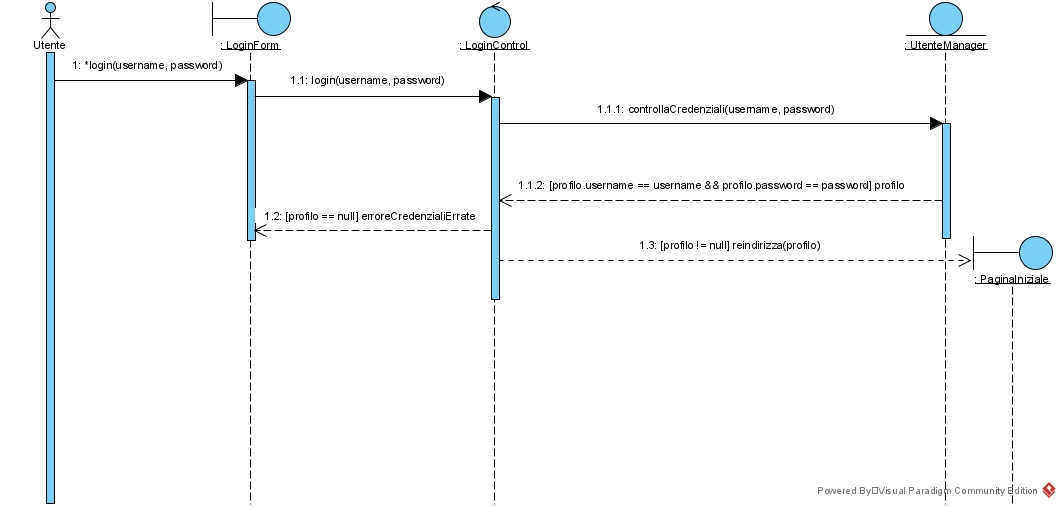
\includegraphics[width=\textwidth,height=\textheight,keepaspectratio]{Figure/SequenceDiagrams/Login.jpg}
\end{center}

\paragraph{Log-out}
\begin{center}
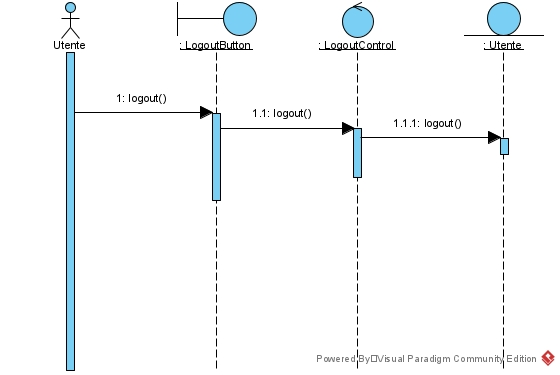
\includegraphics[width=\textwidth,height=\textheight,keepaspectratio]{Figure/SequenceDiagrams/Logout.jpg}
\end{center}

\newpage
\paragraph{Registrazione}
\begin{center}
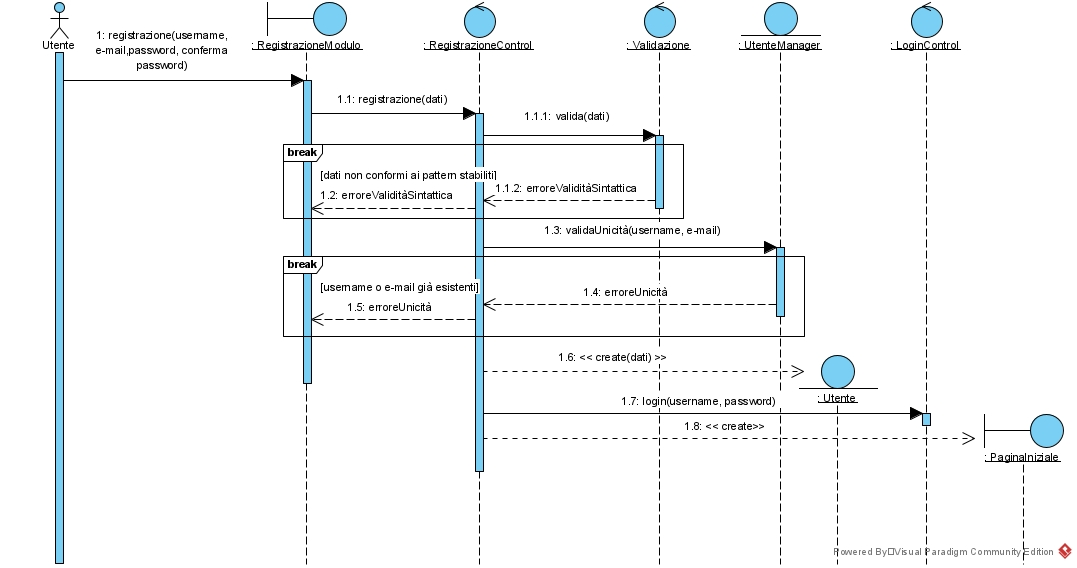
\includegraphics[width=\textwidth,height=\textheight,keepaspectratio]{Figure/SequenceDiagrams/Registrazione.jpg}
\end{center}

\paragraph{Recupero Password}
\begin{center}
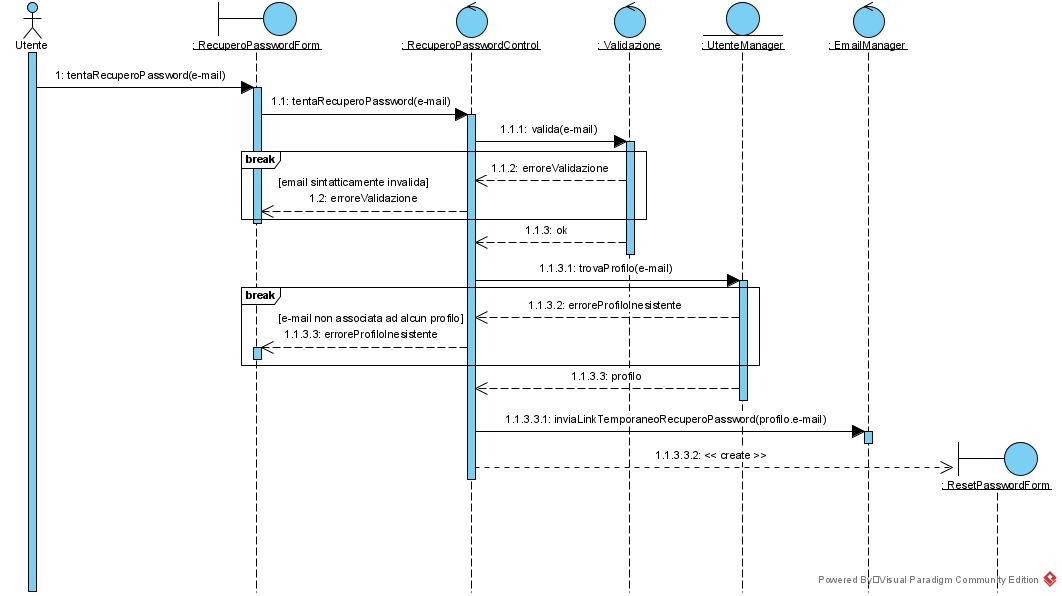
\includegraphics[width=\textwidth,height=\textheight,keepaspectratio]{Figure/SequenceDiagrams/TentaRecuperoPassword.jpg}
\end{center}

\newpage
\begin{center}
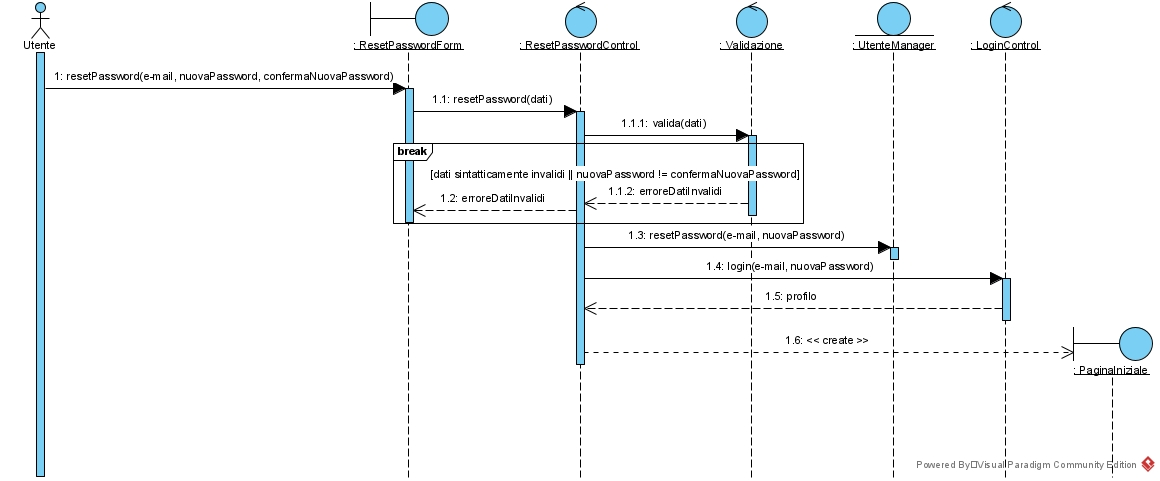
\includegraphics[width=\textwidth,height=\textheight,keepaspectratio]{Figure/SequenceDiagrams/ResetPassword.jpg}
\end{center}

\paragraph{Visualizzazione Profilo}
\begin{center}
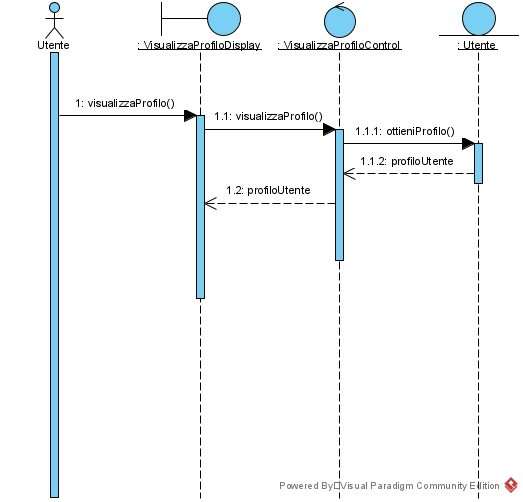
\includegraphics[width=\textwidth,height=\textheight,keepaspectratio]{Figure/SequenceDiagrams/VisualizzazioneProfilo.jpg}
\end{center}

\newpage
\paragraph{Modifica Profilo}
\begin{center}
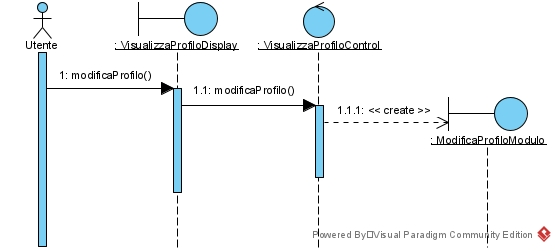
\includegraphics[width=\textwidth,height=\textheight,keepaspectratio]{Figure/SequenceDiagrams/ModificaProfiloEntry.jpg}
\end{center}

\begin{center}
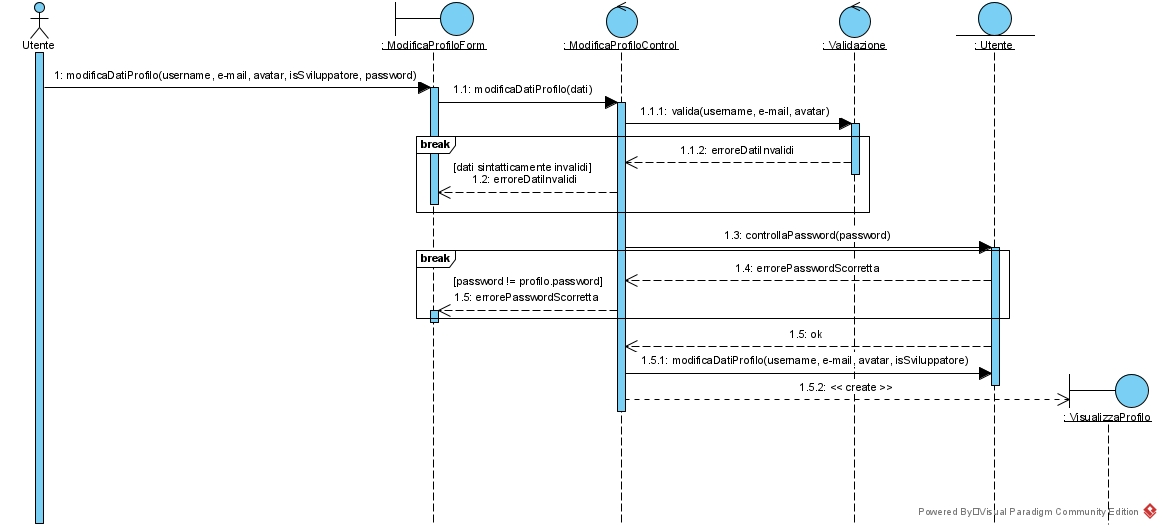
\includegraphics[width=\textwidth,height=\textheight,keepaspectratio]{Figure/SequenceDiagrams/ModificaProfiloInner.jpg}
\end{center}

\newpage
\paragraph{Visualizzazione Dettagli Videogioco}
\begin{center}
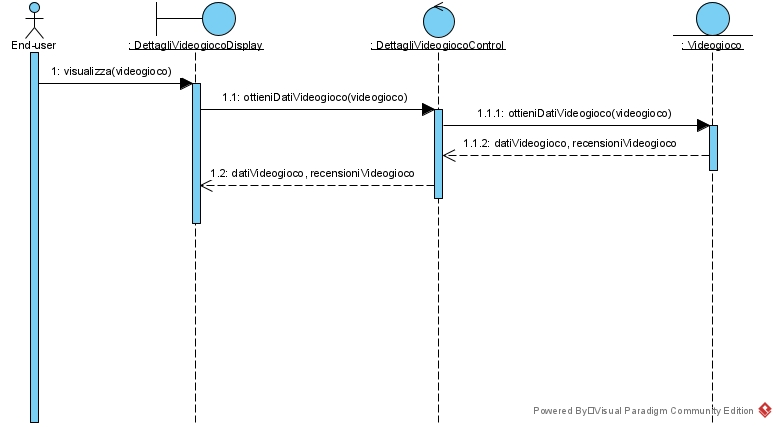
\includegraphics[width=\textwidth,height=\textheight,keepaspectratio]{Figure/SequenceDiagrams/VisualizzazioneDettagliVideogioco.jpg}
\end{center}

\paragraph{Visualizzazione Catalogo}
\begin{center}
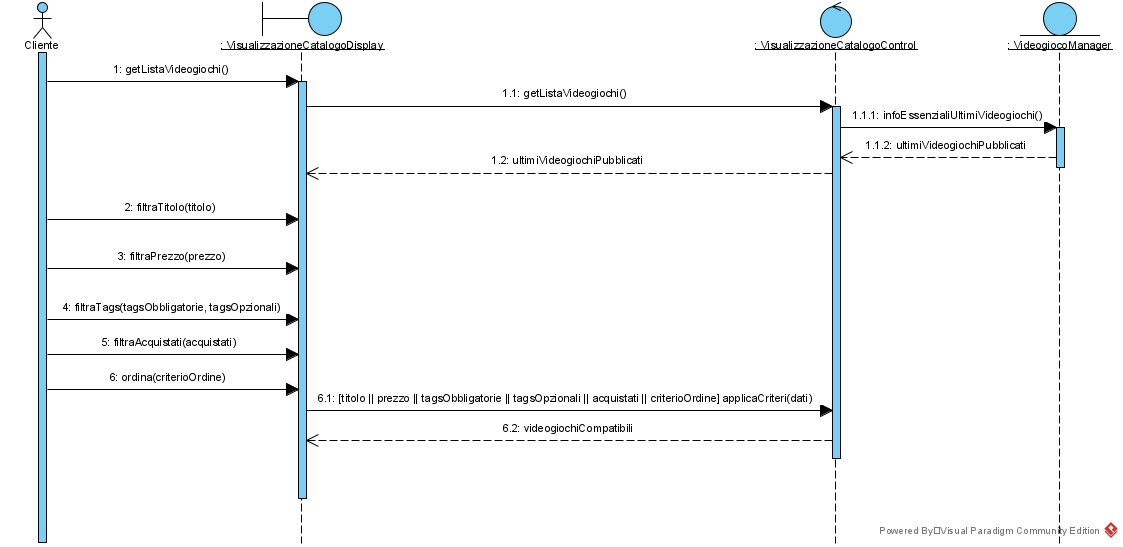
\includegraphics[width=\textwidth,height=\textheight,keepaspectratio]{Figure/SequenceDiagrams/VisualizzazioneCatalogo.jpg}
\end{center}

\newpage
\paragraph{Visualizzazione Pagina Iniziale}
\begin{center}
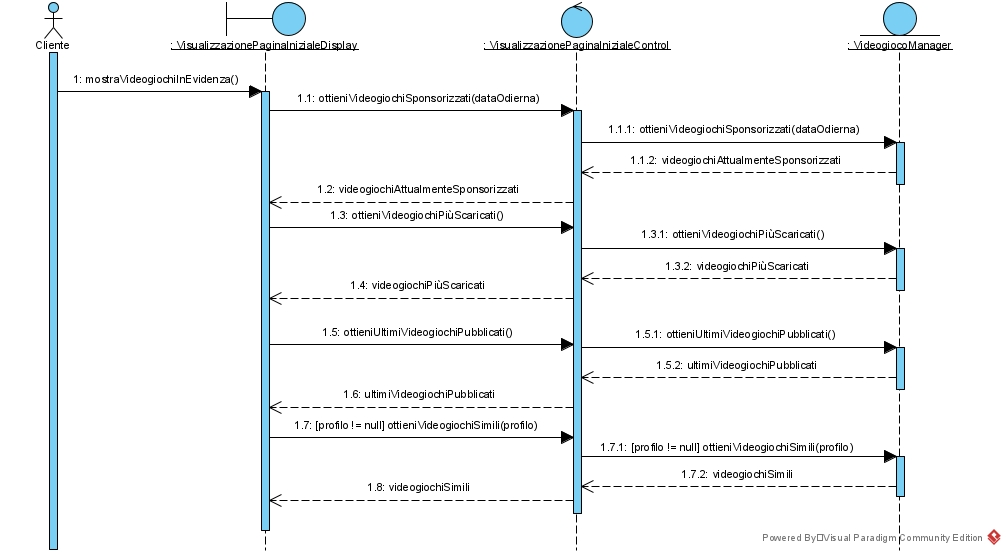
\includegraphics[width=\textwidth,height=\textheight,keepaspectratio]{Figure/SequenceDiagrams/VisualizzazionePaginaIniziale.jpg}
\end{center}

\paragraph{Modifica Dati Videogioco}
\begin{center}
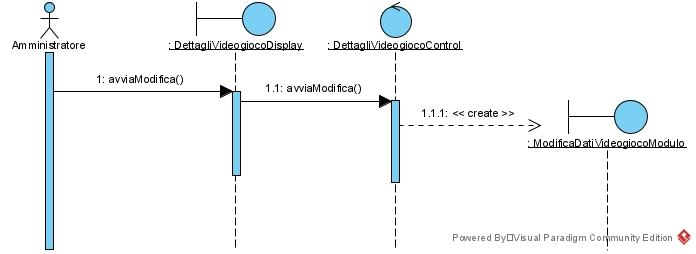
\includegraphics[width=\textwidth,height=\textheight,keepaspectratio]{Figure/SequenceDiagrams/ModificaDatiVideogiocoEntry.jpg}
\end{center}

\newpage
\begin{center}
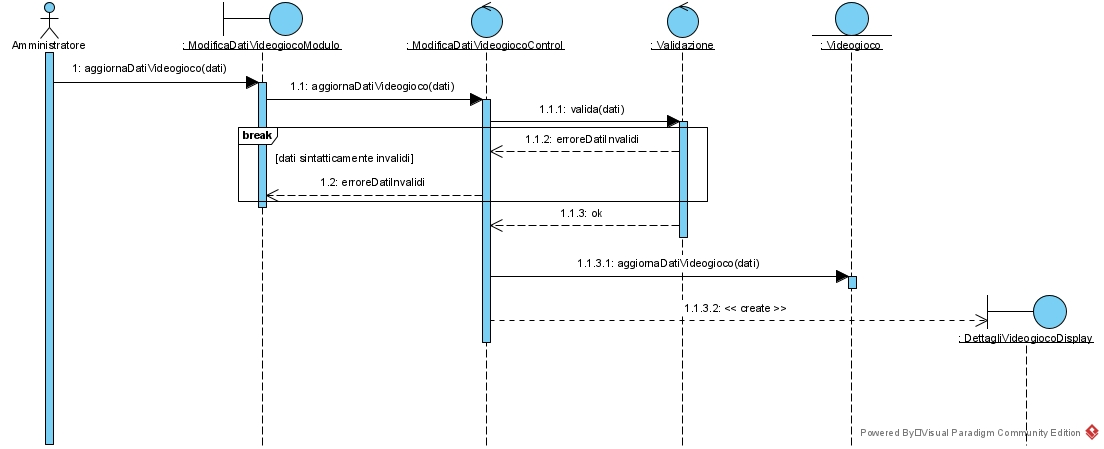
\includegraphics[width=\textwidth,height=\textheight,keepaspectratio]{Figure/SequenceDiagrams/ModificaDatiVideogiocoInner.jpg}
\end{center}

\paragraph{Risoluzione Richiesta Videogioco}
\begin{center}
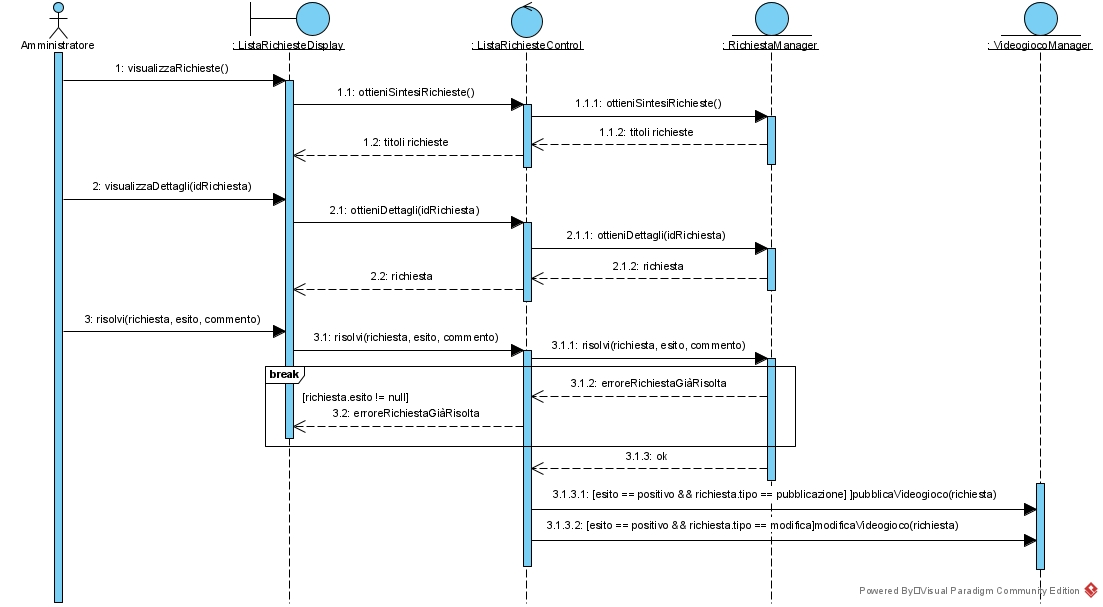
\includegraphics[width=\textwidth,height=\textheight,keepaspectratio]{Figure/SequenceDiagrams/RisoluzioneRichiestaVideogioco.jpg}
\end{center}

\newpage
\paragraph{Richiesta Modifica Videogioco}
\begin{center}
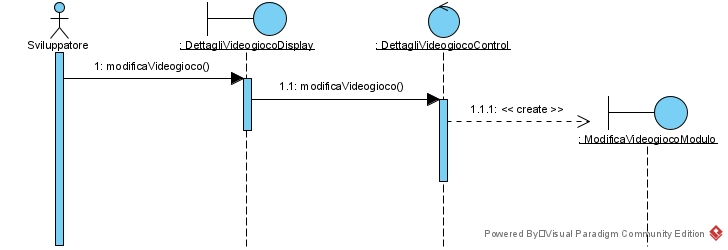
\includegraphics[width=\textwidth,height=\textheight,keepaspectratio]{Figure/SequenceDiagrams/RichiestaModificaVideogiocoEntry.jpg}
\end{center}

\begin{center}
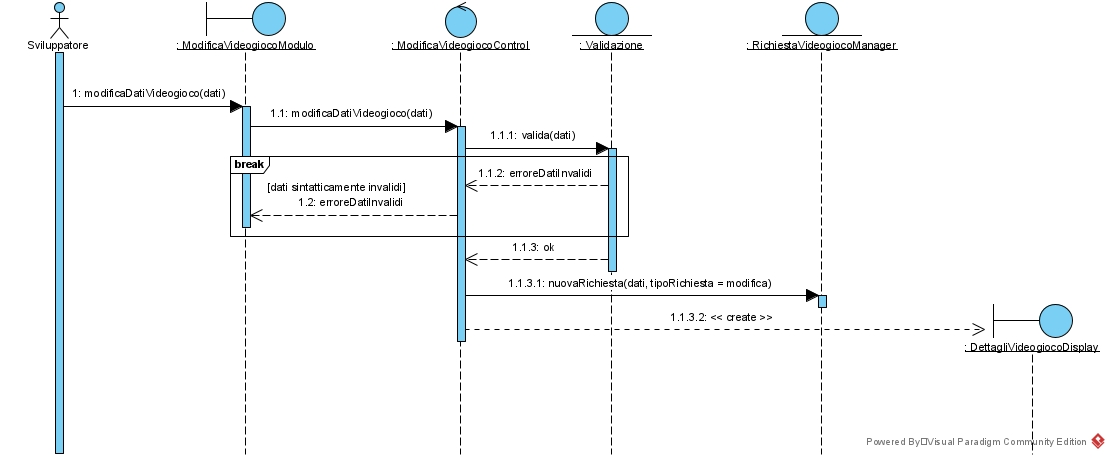
\includegraphics[width=\textwidth,height=\textheight,keepaspectratio]{Figure/SequenceDiagrams/RichiestaModificaVideogiocoInner.jpg}
\end{center}

\newpage
\paragraph{Richiesta Pubblicazione Videogioco}
\begin{center}
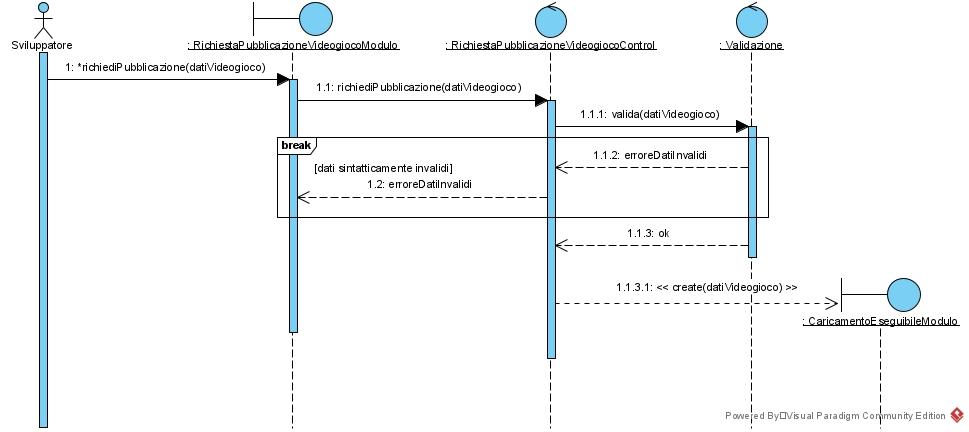
\includegraphics[width=\textwidth,height=\textheight,keepaspectratio]{Figure/SequenceDiagrams/RichiestaPubblicazioneVideogiocoStep1.jpg}
\end{center}

\begin{center}
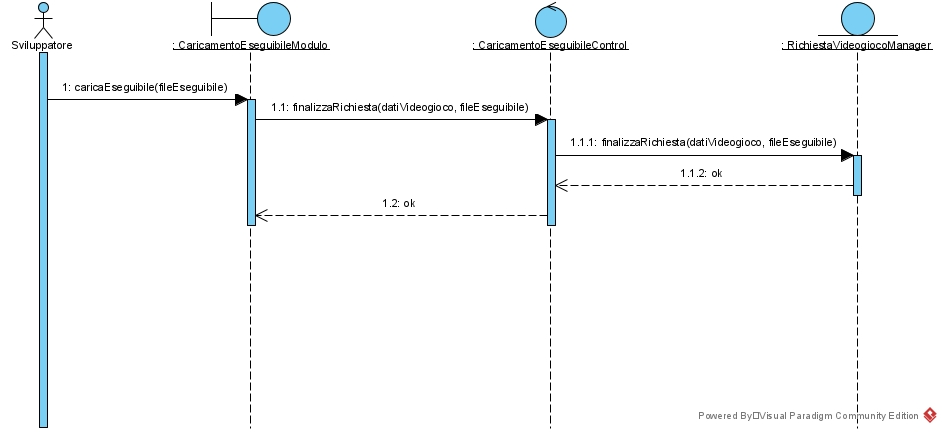
\includegraphics[width=\textwidth,height=\textheight,keepaspectratio]{Figure/SequenceDiagrams/RichiestaPubblicazioneVideogiocoStep2.jpg}
\end{center}

\newpage
\paragraph{Sponsorizzazione Videogioco}
\begin{center}
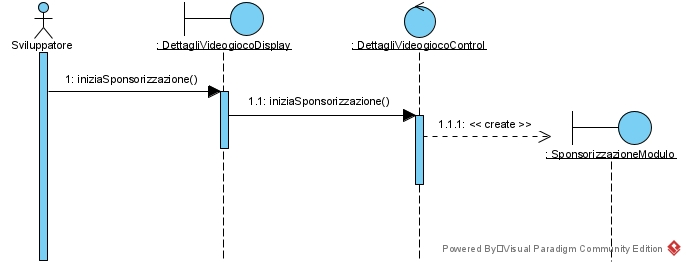
\includegraphics[width=\textwidth,height=\textheight,keepaspectratio]{Figure/SequenceDiagrams/SponsorizzazioneVideogiocoEntry.jpg}
\end{center}

\begin{center}
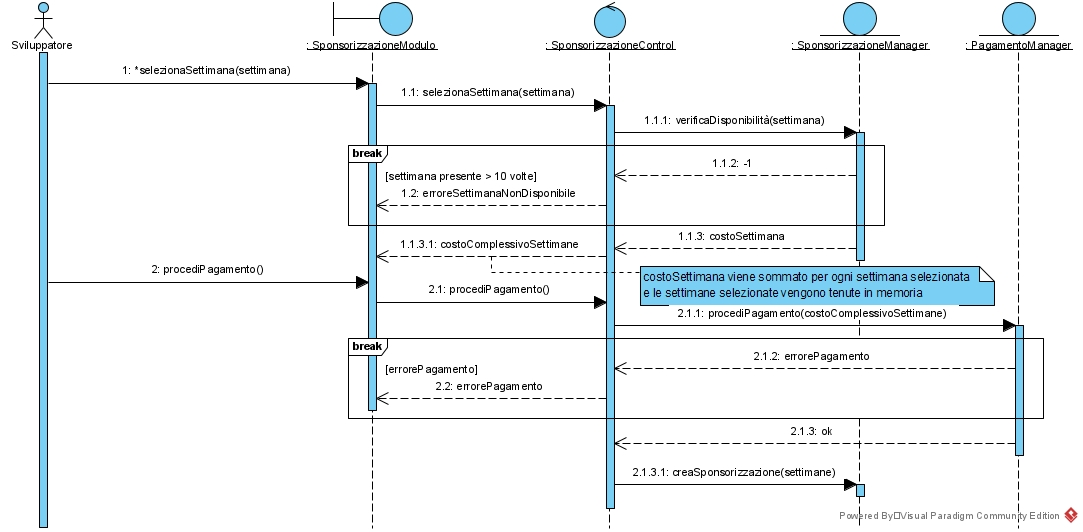
\includegraphics[width=\textwidth,height=\textheight,keepaspectratio]{Figure/SequenceDiagrams/SponsorizzazioneVideogiocoInner.jpg}
\end{center}

\newpage
\paragraph{Acquisto Videogioco}
\begin{center}
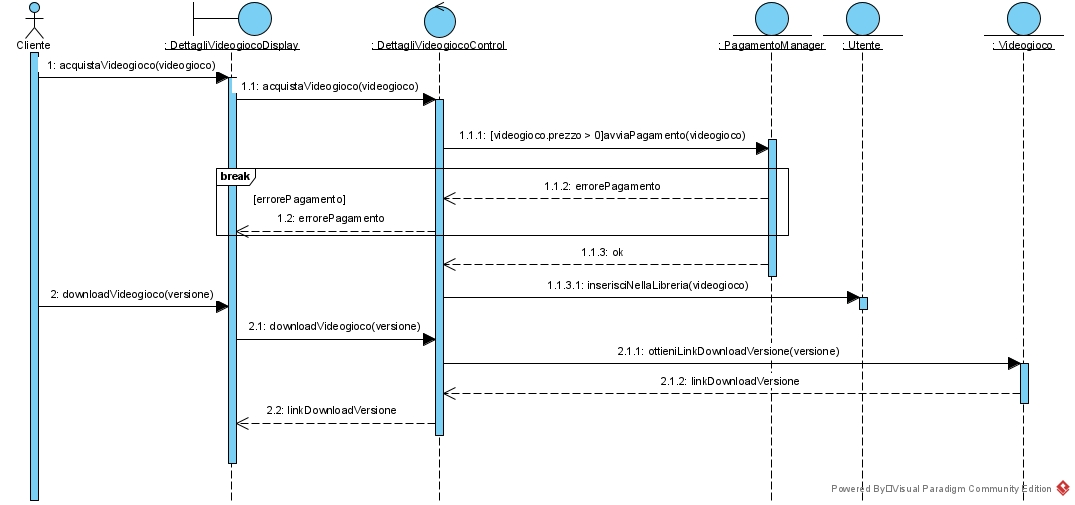
\includegraphics[width=\textwidth,height=\textheight,keepaspectratio]{Figure/SequenceDiagrams/AcquistoVideogioco.jpg}
\end{center}

\paragraph{Suggerimento Tags}
\begin{center}
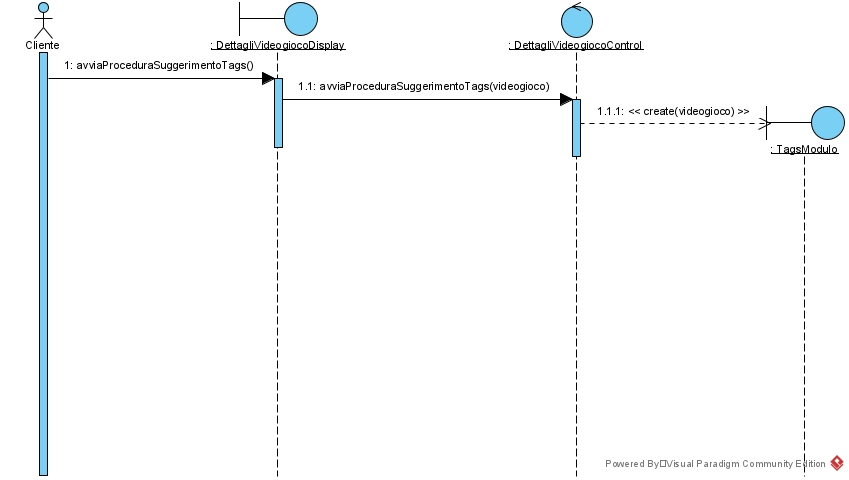
\includegraphics[width=\textwidth,height=\textheight,keepaspectratio]{Figure/SequenceDiagrams/SuggerimentoTagsEntry.jpg}
\end{center}

\newpage
\begin{center}
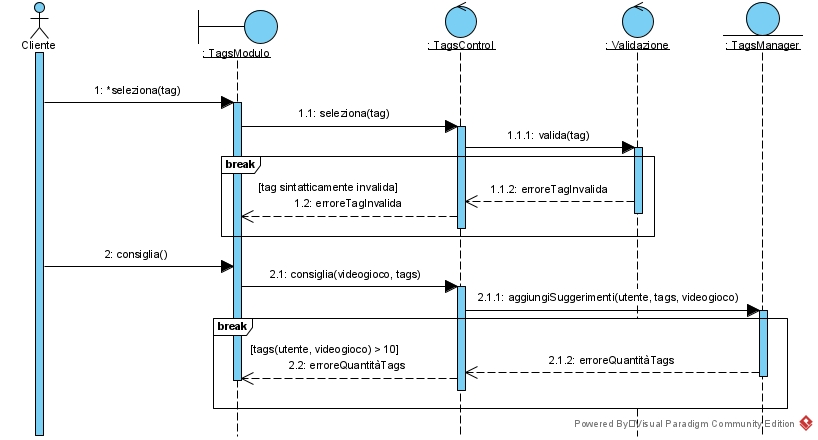
\includegraphics[width=\textwidth,height=\textheight,keepaspectratio]{Figure/SequenceDiagrams/SuggerimentoTagsInner.jpg}
\end{center}

\begin{center}
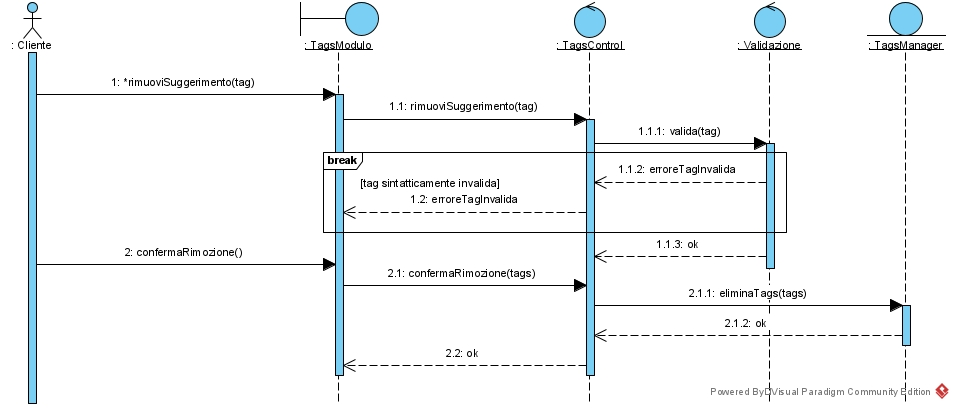
\includegraphics[width=\textwidth,height=\textheight,keepaspectratio]{Figure/SequenceDiagrams/SuggerimentoTagsRemove.jpg}
\end{center}

\newpage
\paragraph{Valutazione Recensione}
\begin{center}
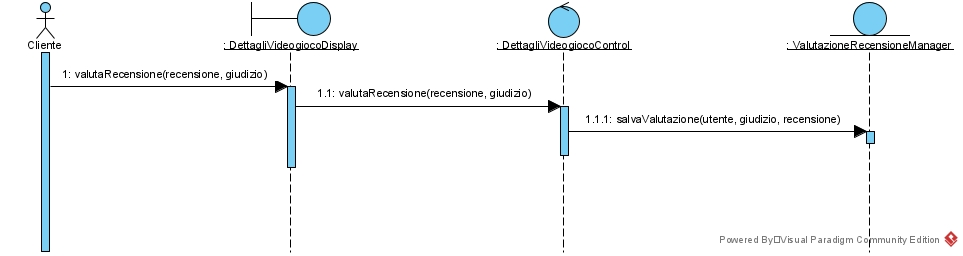
\includegraphics[width=\textwidth,height=\textheight,keepaspectratio]{Figure/SequenceDiagrams/ValutazioneRecensione.jpg}
\end{center}

\paragraph{Recensione Videogioco}
\begin{center}
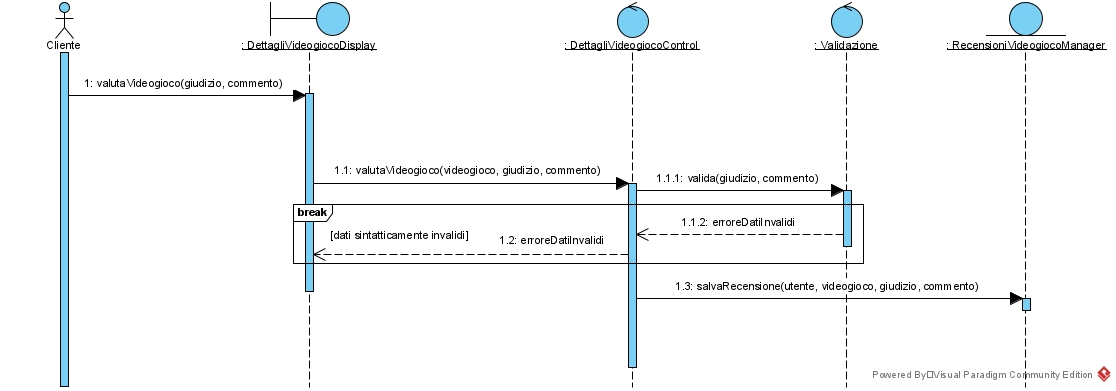
\includegraphics[width=\textwidth,height=\textheight,keepaspectratio]{Figure/SequenceDiagrams/RecensioneVideogioco.jpg}
\end{center}

\newpage
\paragraph{Chiusura Discussione}
\begin{center}
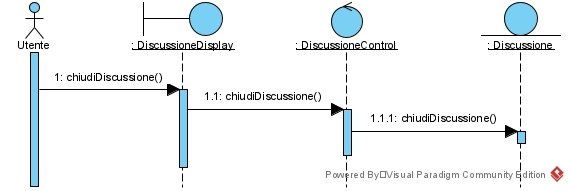
\includegraphics[width=\textwidth,height=\textheight,keepaspectratio]{Figure/SequenceDiagrams/ChiusuraDiscussione.jpg}
\end{center}

\paragraph{Creazione Discussione}
\begin{center}
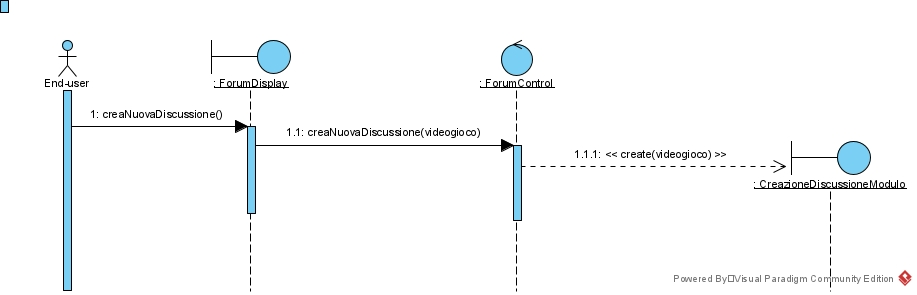
\includegraphics[width=\textwidth,height=\textheight,keepaspectratio]{Figure/SequenceDiagrams/CreazioneDiscussioneEntry.jpg}
\end{center}

\newpage
\begin{center}
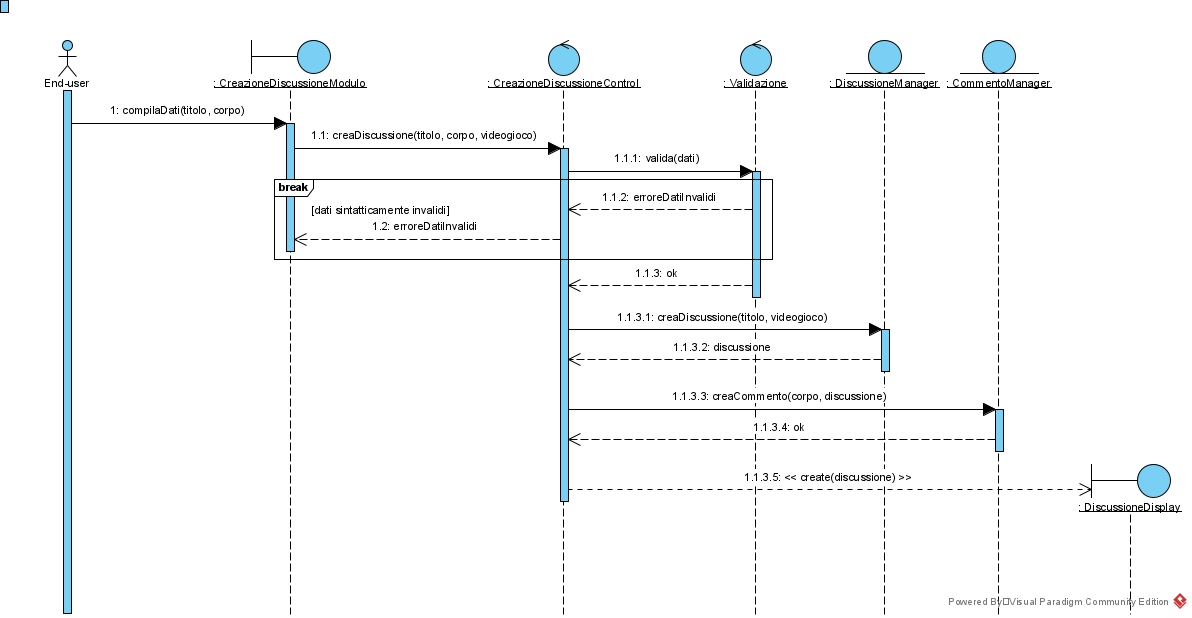
\includegraphics[width=\textwidth,height=\textheight,keepaspectratio]{Figure/SequenceDiagrams/CreazioneDiscussioneInner.jpg}
\end{center}

\paragraph{Commento Discussione}
\begin{center}
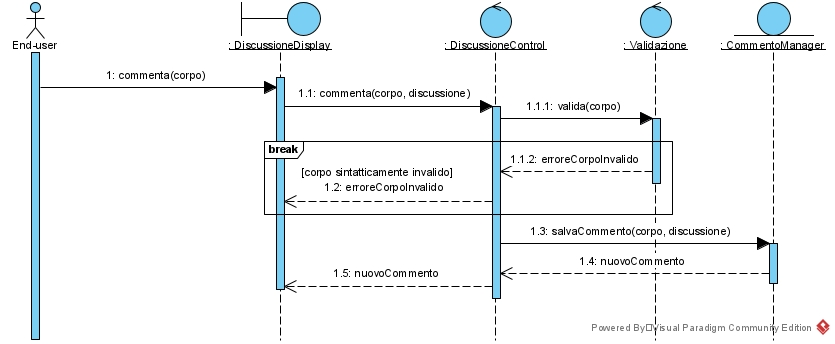
\includegraphics[width=\textwidth,height=\textheight,keepaspectratio]{Figure/SequenceDiagrams/CommentoDiscussione.jpg}
\end{center}

\newpage
\paragraph{Report Contenuto Offensivo}
\begin{center}
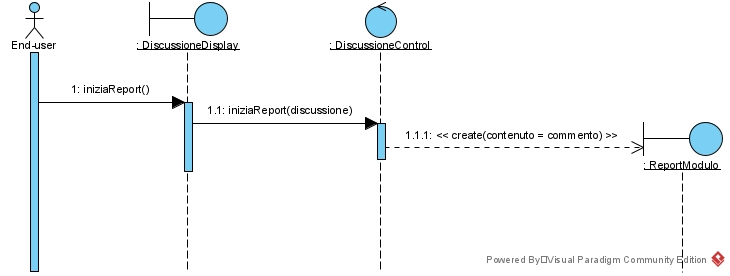
\includegraphics[width=\textwidth,height=\textheight,keepaspectratio]{Figure/SequenceDiagrams/ReportContenutoOffensivoCommento.jpg}
\end{center}

\begin{center}
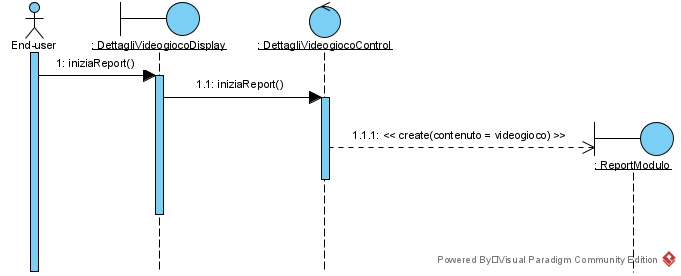
\includegraphics[width=\textwidth,height=\textheight,keepaspectratio]{Figure/SequenceDiagrams/ReportContenutoOffensivoVideogioco.jpg}
\end{center}

\newpage
\begin{center}
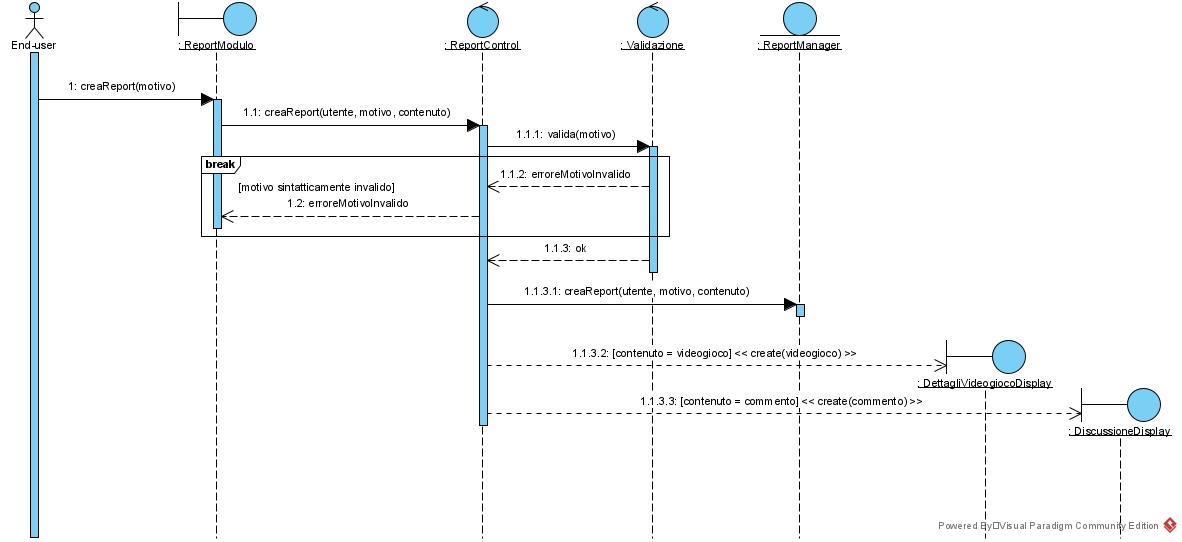
\includegraphics[width=\textwidth,height=\textheight,keepaspectratio]{Figure/SequenceDiagrams/ReportContenutoOffensivoInnerXX.jpg}
\end{center}

\paragraph{Messa in Rilievo di una Discussione}
\begin{center}
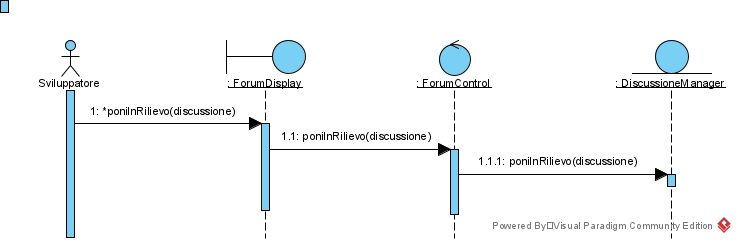
\includegraphics[width=\textwidth,height=\textheight,keepaspectratio]{Figure/SequenceDiagrams/MessaRilievoDiscussione.jpg}
\end{center}

\newpage
\paragraph{Rimozione Contenuto Offensivo}
\begin{center}
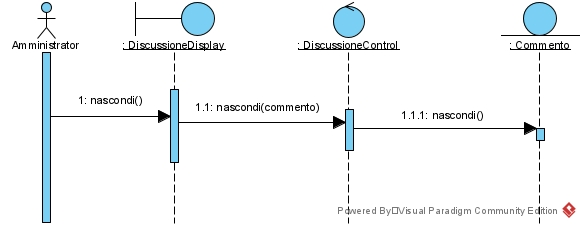
\includegraphics[width=\textwidth,height=\textheight,keepaspectratio]{Figure/SequenceDiagrams/RimozioneContenutoOffensivo.jpg}
\end{center}

\begin{center}
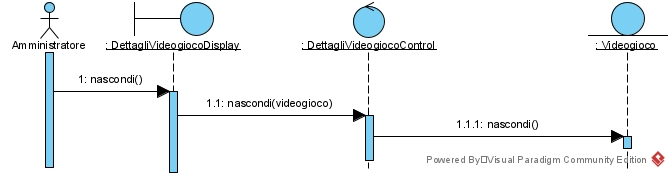
\includegraphics[width=\textwidth,height=\textheight,keepaspectratio]{Figure/SequenceDiagrams/RimozioneContenutoOffensivoVideogioco.jpg}
\end{center}

\newpage
\paragraph{Risoluzione Report}
\begin{center}
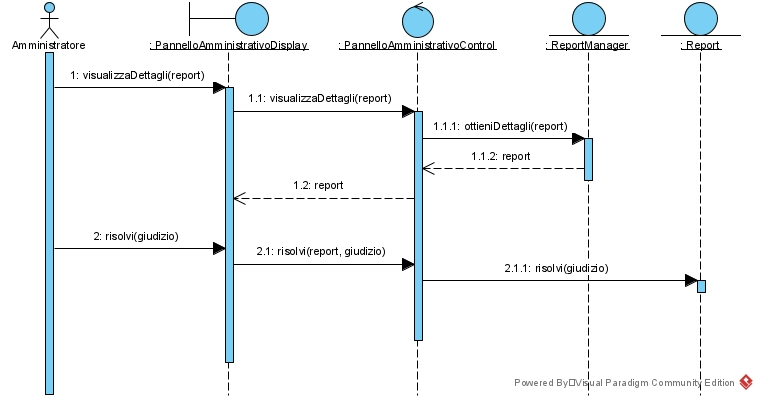
\includegraphics[width=\textwidth,height=\textheight,keepaspectratio]{Figure/SequenceDiagrams/RisoluzioneReport.jpg}
\end{center}



\newpage
\subsection{Diagramma degli stati}
\paragraph{Videogioco}
\begin{center}
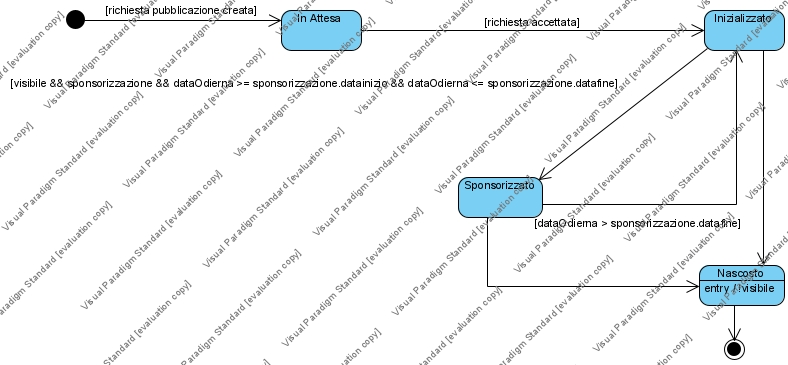
\includegraphics[width=\textwidth,height=\textheight,keepaspectratio]{Figure/StateDiagrams/Videogioco.jpg}
\end{center}

\paragraph{Discussione}
\begin{center}
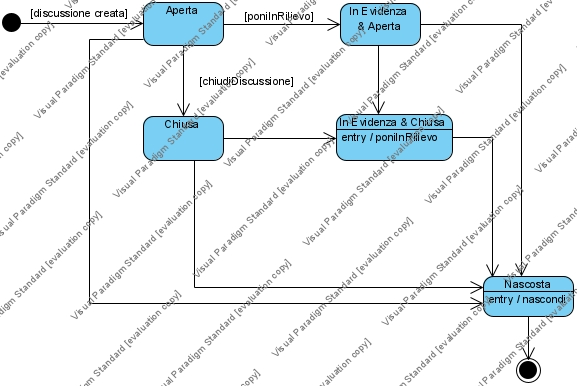
\includegraphics[width=\textwidth,height=\textheight,keepaspectratio]{Figure/StateDiagrams/Discussione.jpg}
\end{center}

\newpage
\paragraph{Richiesta}
\begin{center}
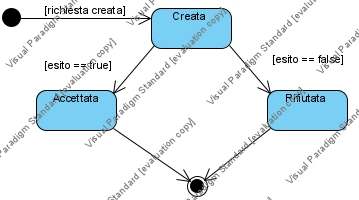
\includegraphics[width=\textwidth,height=\textheight,keepaspectratio]{Figure/StateDiagrams/Richiesta.jpg}
\end{center}

\subsection{Diagramma di Navigazione}
\begin{center}
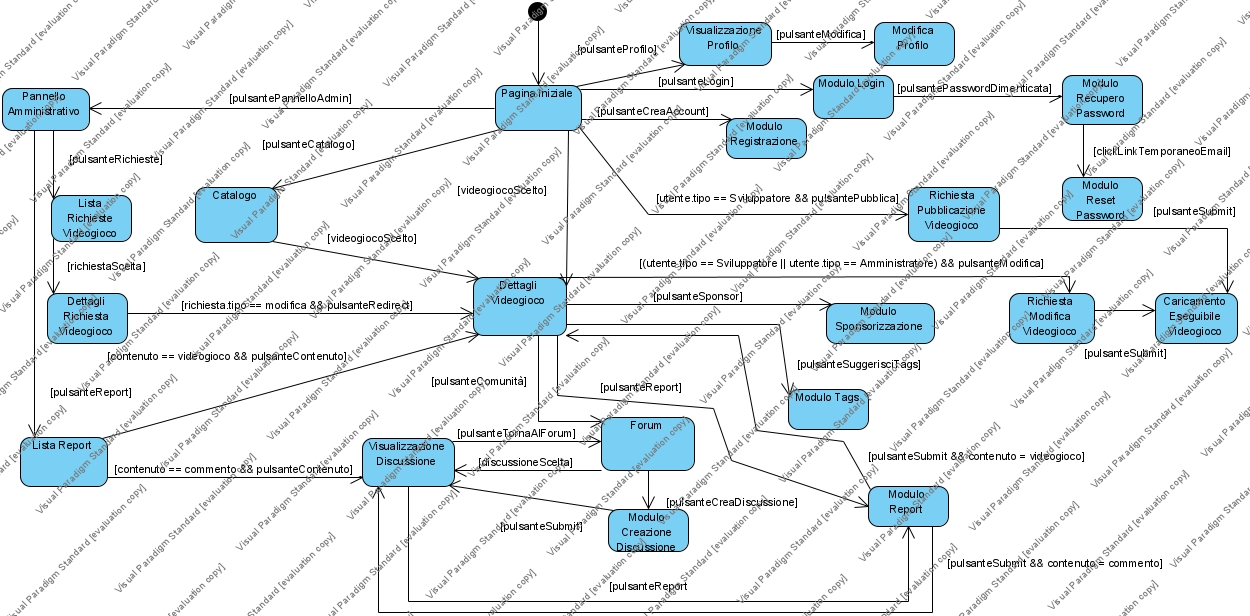
\includegraphics[width=\textwidth,height=\textheight,keepaspectratio]{Figure/NavigationalPath.jpg}
\end{center}

\newpage
\subsection{Mockups}
\paragraph{Pagina Iniziale}
\begin{center}
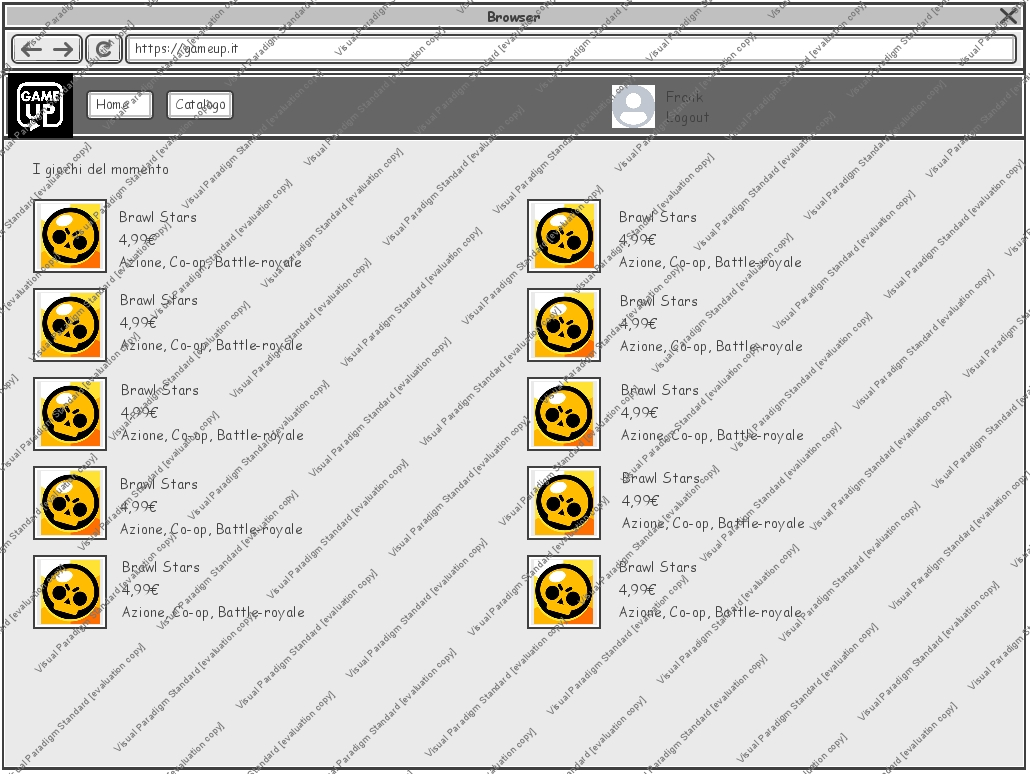
\includegraphics[width=\textwidth,height=\textheight,keepaspectratio]{Figure/Mockups/PaginaIniziale.jpg}
\end{center}

\newpage
\paragraph{Catalogo}
\begin{center}
\includegraphics[width=\textwidth,height=\textheight,keepaspectratio]{Figure/Mockups/Catalogo.jpg}
\end{center}

\newpage
\paragraph{Dettagli Videogioco}
\begin{center}
\includegraphics[width=\textwidth,height=\textheight,keepaspectratio]{Figure/Mockups/DettagliVideogioco.jpg}
\end{center}

\newpage
\paragraph{Visualizza Profilo}
\begin{center}
\includegraphics[width=\textwidth,height=\textheight,keepaspectratio]{Figure/Mockups/VisualizzaProfilo.jpg}
\end{center}

\newpage
\paragraph{Modifica Profilo}
\begin{center}
\includegraphics[width=\textwidth,height=\textheight,keepaspectratio]{Figure/Mockups/ModificaProfilo.jpg}
\end{center}

\newpage
\paragraph{Log-in}
\begin{center}
\includegraphics[width=\textwidth,height=\textheight,keepaspectratio]{Figure/Mockups/Login.jpg}
\end{center}

\newpage
\paragraph{Recupero Password}
\begin{center}
\includegraphics[width=\textwidth,height=\textheight,keepaspectratio]{Figure/Mockups/RecuperoPassword1.jpg}
\end{center}

\newpage
\begin{center}
\includegraphics[width=\textwidth,height=\textheight,keepaspectratio]{Figure/Mockups/RecuperoPassword2.jpg}
\end{center}

\newpage
\paragraph{Registrazione}
\begin{center}
\includegraphics[width=\textwidth,height=\textheight,keepaspectratio]{Figure/Mockups/Registrazione.jpg}
\end{center}

\newpage
\paragraph{Richiesta Pubblicazione Videogioco}
\begin{center}
\includegraphics[width=\textwidth,height=\textheight,keepaspectratio]{Figure/Mockups/RichiestaPubblicazioneVideogioco1.jpg}
\end{center}

\newpage
\begin{center}
\includegraphics[width=\textwidth,height=\textheight,keepaspectratio]{Figure/Mockups/RichiestaPubblicazioneVideogioco2.jpg}
\end{center}

\newpage
\paragraph{Richiesta Modifica Videogioco}
\begin{center}
\includegraphics[width=\textwidth,height=\textheight,keepaspectratio]{Figure/Mockups/RichiestaModificaVideogioco.jpg}
\end{center}

\newpage
\begin{center}
\includegraphics[width=\textwidth,height=\textheight,keepaspectratio]{Figure/Mockups/RichiestaPubblicazioneVideogioco2.jpg}
\end{center}

\newpage
\paragraph{Sponsorizzazione Videogioco}
\begin{center}
\includegraphics[width=\textwidth,height=\textheight,keepaspectratio]{Figure/Mockups/SponsorizzaVideogioco.jpg}
\end{center}

\newpage
\paragraph{Suggerimento Tags}
\begin{center}
\includegraphics[width=\textwidth,height=\textheight,keepaspectratio]{Figure/Mockups/SuggerimentoTags.jpg}
\end{center}

\newpage
\paragraph{Report Contenuto Offensivo}
\begin{center}
\includegraphics[width=\textwidth,height=\textheight,keepaspectratio]{Figure/Mockups/Report.jpg}
\end{center}

\newpage
\paragraph{Forum}
\begin{center}
\includegraphics[width=\textwidth,height=\textheight,keepaspectratio]{Figure/Mockups/Forum.jpg}
\end{center}

\newpage
\paragraph{Creazione Discussione}
\begin{center}
\includegraphics[width=\textwidth,height=\textheight,keepaspectratio]{Figure/Mockups/CreazioneDiscussione.jpg}
\end{center}

\newpage
\paragraph{Richiesta Modifica Videogioco}
\begin{center}
\includegraphics[width=\textwidth,height=\textheight,keepaspectratio]{Figure/Mockups/RichiestaModificaVideogioco.jpg}
\end{center}

\newpage
\paragraph{Visualizzazione Discussione}
\begin{center}
\includegraphics[width=\textwidth,height=\textheight,keepaspectratio]{Figure/Mockups/Discussione.jpg}
\end{center}

\newpage
\paragraph{Lista Report}
\begin{center}
\includegraphics[width=\textwidth,height=\textheight,keepaspectratio]{Figure/Mockups/DettagliReport.jpg}
\end{center}

\newpage
\paragraph{Lista Richieste}
\begin{center}
\includegraphics[width=\textwidth,height=\textheight,keepaspectratio]{Figure/Mockups/ListaRichiesteVideogioco.jpg}
\end{center}

\newpage
\paragraph{Dettagli Richiesta}
\begin{center}
\includegraphics[width=\textwidth,height=\textheight,keepaspectratio]{Figure/Mockups/DettagliRichiesta.jpg}
\end{center}

\newpage
\subsection{Glossario}
\begin{itemize}
	\item End-User: Un utente target del sistema, ovvero un cliente oppure uno sviluppatore;
	\item Forum: Spazio condiviso da sviluppatori e clienti con un interesse in comune, ovvero un particolare videogioco, per favorirne l’interazione;
	\item Report: Segnalazione creata da un utente per notificare gli amministratori della piattaforma di un contenuto non consono, che non rispetta le linee guida definite e rese pubbliche;
	\item Tag: Una singola parola o un insieme di poche parole che descrivono sinteticamente una caratteristica particolare di un videogioco;
	\item Versione Videogioco: Una istantanea di un videogioco in un particolare momento o periodo, resa pubblica per permetterne il download e con una particolare dicitura testuale che ne specifica il tipo di differenza rispetto alle altre istantanee esistenti, ovvero se comprende cambiamenti minimi (che variano leggermente alcune caratteristiche del videogioco stesso) o significativi;
	\item Videogioco: Un software che simula situazioni di carattere ludico, permettendo ad uno o più giocatori di interagire tra di loro e/o con la simulazione tramite un dispositivo elettronico, nel caso di questo documento principalmente dispositivi mobili;
\end{itemize}